\documentclass[sigconf,nonacm]{acmart}
\usepackage{booktabs}
\usepackage{multirow}
\usepackage{graphicx}
\usepackage{tikz}
\usetikzlibrary{positioning,arrows.meta,calc}
\usepackage{subcaption}
\usepackage{hyperref}
\usepackage{algorithm}
\usepackage{algpseudocode}
\usepackage{amsmath}

\newcommand{\best}[1]{\textbf{#1}}
\newcommand{\second}[1]{\underline{#1}}

%%
%% Remove ACM-specific publication information
%%
\settopmatter{
    printacmref=false,
    printfolios=false
}

%%
%% Title
%%
% \title{Multipath in Satellite-Terrestrial Integrated Networks \\ for Real-Time Applications}
\title{Prediction Aware Multipath Scheduling in\\Satellite--Terrestrial Integrated Networks\\for Real-Time Applications}
  \author{
    Evan Gossling, Jalal Jalali, Daji Qiao, Hongwei Zhang
    \\
    \textit{Iowa State University}
    \\[1em]
    Naveen Rajanikantha, Ben Haan, Andrew Bys
    \\
    \textit{Collins Aerospace}
}

%%
%% Short author list for headers
%% TODO Change for publication
%%
\renewcommand{\shortauthors}{Copyright © 2026 Center for Wireless, Communities and Innovation (WiCI)}

\begin{document}

\begin{abstract}
Integrated terrestrial and LEO satellite networks provide complementary connectivity for real-time applications, but their heterogeneous and time-varying path conditions make reactive multipath scheduling difficult. This work investigates prediction-aware packet scheduling using a Multipath QUIC-based \emph{liquid tunnel} that combines path telemetry with temporal predictions of RTT, throughput, and packet loss. We evaluate conventional minRTT scheduling, a predictive-minRTT scheduler, and a QoE-predictive scheduler over 5G and Starlink uplinks using a 4K 30~FPS video stream. Results show that prediction improves application performance even when applied to a basic scheduling policy: predictive-minRTT reduces frame loss per second by 52\% compared with conventional minRTT. The QoE-predictive scheduler further achieves the highest average FPS (27.05), lowest frame loss (0.90 frames/s), and lowest total frame loss (54 frames), although it exhibits higher packet loss and requires further refinement to address reordering and visual artifacts. These results demonstrate the potential of prediction-aware multipath scheduling while highlighting the remaining challenges of robust packet-level traffic steering in heterogeneous terrestrial--satellite networks.
\end{abstract}

\maketitle

% \tableofcontents

\section{Introduction}


% \begin{table}[t]
% \centering
% \caption{List of Abbreviations}
% \label{tab:abbreviations}
% \renewcommand{\arraystretch}{1.10}
% \setlength{\tabcolsep}{5pt}
% \begin{tabular}{lp{5.2cm}}
% \toprule
% \textbf{Abbreviation} & \textbf{Definition} \\
% \midrule
% 3GPP    & Third Generation Partnership Project \\
% 5G      & Fifth-Generation Mobile Network \\
% API     & Application Programming Interface \\
% ARA     & ARA Wireless Living Lab \\
% BS      & Base Station \\
% CID     & Connection ID \\
% COTS    & Commercial Off-the-Shelf \\
% CPU     & Central Processing Unit \\
% DL      & Downlink \\
% DTC     & Direct-to-Cell \\
% EMA     & Exponential Moving Average \\
% FEC     & Forward Error Correction \\
% FPS     & Frames Per Second \\
% G/G/1   & General-Arrival/General-Service Single-Server Queue \\
% GPU     & Graphics Processing Unit \\
% gRPC    & Google Remote Procedure Call \\
% GRU     & Gated Recurrent Unit \\
% IFA     & Inter-Frame Arrival \\
% I/O     & Input/Output \\
% IP      & Internet Protocol \\
% JSON    & JavaScript Object Notation \\
% LEO     & Low-Earth Orbit \\
% LTS     & Long-Term Support \\
% ML      & Machine Learning \\
% MPQUIC  & Multipath QUIC \\
% MPTCP   & Multipath TCP \\
% NTN     & Non-Terrestrial Network \\
% PC      & Personal Computer \\
% PoP     & Point of Presence \\
% QoE     & Quality of Experience \\
% QoS     & Quality of Service \\
% QUIC    & QUIC Transport Protocol \\
% RAM     & Random-Access Memory \\
% RAN     & Radio Access Network \\
% RFC     & Request for Comments \\
% RSRP    & Reference Signal Received Power \\
% RSRQ    & Reference Signal Received Quality \\
% RTP     & Real-Time Transport Protocol \\
% RTT     & Round-Trip Time \\
% RTTVAR  & Round-Trip Time Variation \\
% Seq2Seq & Sequence-to-Sequence \\
% SINR    & Signal-to-Interference-plus-Noise Ratio \\
% STIN    & Satellite--Terrestrial Integrated Network \\
% TCP     & Transmission Control Protocol \\
% TVWS    & TV White Space \\
% UDP     & User Datagram Protocol \\
% UE      & User Equipment \\
% UL      & Uplink \\
% UT      & User Terminal \\
% VM      & Virtual Machine \\
% \bottomrule
% \end{tabular}
% \end{table}

\subsection{Key Insights}
% For Collins report only
The evaluation of the proposed liquid tunnel provides several key insights into the use of multipath communication, path prediction, and intelligent packet scheduling in satellite--terrestrial integrated networks. In particular, we demonstrate the benefits of combining heterogeneous paths and incorporating predicted network conditions into packet-scheduling decisions for real-time applications. At the same time, the evaluation identifies further development, particularly with respect to packet loss, packet reordering, path-model accuracy, and the integration of FEC into the scheduling process. The main findings and directions for future development are summarized as follows:

\begin{itemize}
    \item \textbf{Multipath increases application QoE:} utilizing multipath, even in a very heterogeneous network environment such as a satellite--terrestrial integrated network, improves application performance.
    \item \textbf{Path modeling increases application QoE:} integrating path models into a multipath scheduler allows the scheduler to make more proactive scheduling decisions. Our results showcase better application performance with our predictive-minRTT, which incorporates path models, over the default minRTT scheduling algorithm.
    \item \textbf{Intelligent scheduling algorithms increase application QoE:} our QoE-Predictive scheduling algorithm outperforms the baseline minRTT and the predictive-minRTT, providing higher average FPS and reducing the frame losses by $49.5\%-92.4\%$ compared to the other scheduling methods.
    \item \textbf{Improve our intelligent scheduling algorithm:} while our scheduling algorithm provided better application performance, we observed a high amount of packet loss and an occasional spike in packet reordering. Furthermore, while the video frames are fresher, we visually note some significant visual artifacting and discoloration in the video stream. Therefore, we need to further refine the algorithm for the final deliverable to improve these aspects.
    \item \textbf{Improve our path models:} we plan to further develop and train our path models so that they can provide even greater benefits to our scheduler and the liquid tunnel.
    \item \textbf{FEC integration uses RaptorQ erasure coding:} while FEC is integrated into our liquid tunnel, we did not utilize it in this report. For our next deliverable, we plan to use RaptorQ erasure coding as well as integrate it into the scheduler, not just the liquid tunnel. In this manner, the scheduler can have a direct understanding of which packets belong to which block, which will have a high impact on FEC performance.
    
\end{itemize}


\subsection{Problem Statement}

In a satellite--terrestrial integrated network (STIN), each available path $i \in \mathcal{P}$ exhibits time-varying RTT, throughput, and packet-loss characteristics. At each packet transmission time $t$, the scheduler must select a path that minimizes the expected delivery cost despite only having access to imperfect observations of the current path state. Let the observed state be
\[
\mathbf{s}_i(t) =
\left[R_i(t), B_i(t), L_i(t)\right],
\]
and the predicted future state over horizon $\tau$ be
\[
\hat{\mathbf{s}}_i(t+\tau) =
\left[\hat{R}_i(t+\tau),\hat{B}_i(t+\tau),\hat{L}_i(t+\tau)\right].
\]
A conventional scheduler selects a path using $\mathbf{s}_i(t)$, whereas a prediction-aware scheduler can incorporate $\hat{\mathbf{s}}_i(t+\tau)$ to account for anticipated path degradation or improvement. The scheduling problem is therefore to determine whether a predicted path state can produce better packet-level decisions than reactive state alone, and how such predictions should be incorporated to improve real-time application QoE while limiting packet loss, delay, and reordering.

\section{Liquid Tunnel}
\label{sec:liquid_tunnel}

To evaluate intelligent multipath scheduling over heterogeneous satellite-terrestrial networks, we employ a \emph{liquid tunnel} as our end-to-end transport framework between our client and server. The liquid tunnel provides a unified logical connection over physically distinct access networks, allowing easy integration with our applications so we may dynamically distribute their traffic between terrestrial and satellite networks. 

% In the considered architecture, the available paths may include terrestrial 5G connectivity together with LEO satellite links such as Starlink and OneWeb. 

% Rather than exposing these heterogeneous links directly to the application, Liquid Tunnel abstracts them as a single communication tunnel and performs path selection and packet scheduling within the transport framework.

This abstraction towards a single communication tunnel is particularly important for our transport architecture as the available paths exhibit substantially different time-varying characteristics. 
% TODO move to intro/motivation citing Starlink and explaining recofig at set inervals every 15s (cite paper) and cite ARA studies for 5G dynamics
% Terrestrial and LEO satellite links differ not only in their average latency and capacity but also in the mechanisms responsible for short-term performance variations. Starlink exhibits satellite- and network-reconfiguration dynamics, whereas terrestrial 5G links are affected primarily by radio conditions, interference, resource allocation, and network load. 
Consequently, selecting an incorrect path, or path based only on its instantaneous state, may cause frequent path switching, packet reordering, or the selection of a path whose performance is about to deteriorate. All of these factors will contribute to multipath performance degradation due to out-of-order packet arrivals or high overhead from path switching.

By abstracting the transport layer for the application, the liquid tunnel can improve application QoE by providing path management, intelligent packet steering, path prediction via integrated modeling, and increased reliability with erasure coding.
% The liquid tunnel therefore provides the execution layer through which the prediction models developed in this work can ultimately influence packet transmission. The objective is to move from conventional \emph{reactive} multipath scheduling, in which packets are assigned according to currently observed network conditions, toward \emph{prediction-in-the-loop} scheduling, in which short-term forecasts of path conditions are incorporated into scheduling decisions. In particular, predictions of RTT, throughput, and packet loss can provide the scheduler with information regarding the expected future state of each available path. This enables the scheduler to preferentially transmit latency-sensitive traffic over paths expected to remain stable while reducing traffic allocation to paths predicted to experience degradation.

\subsection{Transport Architecture}
\label{subsec:transport_architecture}

% The Liquid Tunnel architecture separates application communication from the underlying access networks. An application generates traffic toward a remote endpoint through a logical tunnel, while Liquid Tunnel maintains connectivity over the available physical network interfaces. Each interface constitutes a candidate transport path and may exhibit a different combination of latency, throughput, packet loss, and available capacity.

% For the satellite-terrestrial scenario considered in this work, the architecture can simultaneously expose a terrestrial 5G path and one or more LEO satellite paths to the transport layer. The 5G path traverses the UE, the terrestrial RAN, and the 5G core before reaching the remote endpoint. In contrast, a Starlink path traverses the user terminal (UT), serving satellite, ground station (GS), Starlink Point of Presence (PoP), and the public Internet. These differences create heterogeneous end-to-end path characteristics even when the paths terminate at the same application server.

% At the sender, Liquid Tunnel receives application packets and assigns them to one of the available paths according to the active scheduling policy. Each path is continuously characterized using network measurements such as RTT, throughput, packet loss, and throughput. These measurements provide the scheduler with information about the current network state and also serve as inputs to the temporal prediction models developed in this work. At the receiver, traffic arriving over the different paths is presented through the common tunnel abstraction, thereby hiding the underlying path diversity from the application.

% This architecture enables the scheduling mechanism to operate independently of the application while retaining visibility into path-specific network conditions. Such separation is particularly useful for real-time applications, where changing the application itself to account for individual satellite and terrestrial links would be undesirable. Instead, path heterogeneity can be managed within the transport layer.

% \begin{figure*}[t]
% \centering
% \resizebox{0.78\textwidth}{!}{%
%     \input{images/tun_ip_stack}
% }
% \caption{Architecture of the liquid tunnel protocol stack, illustrating the virtual tunnel interface, MPQUIC control and data planes, path monitoring and metrics, optional FEC and modeling components, multipath scheduling, and the underlying physical network interfaces.}
% \label{fig:tun_ip_stack}
% \end{figure*}

\subsubsection{Protocol}
\label{subsubsec:liquid_protocol}

Our liquid tunnel utilizes multipath QUIC (MPQUIC) as its base transport protocol, one of the three 3GPP protocols for Access Traffic Steering, Switching, and Splitting \cite{10.1109/MCOMSTD.0006.2200056, 3gpp2024atsss}. We choose QUIC as it provides a user-space transport protocol built on UDP and integrates end-to-end reliability, congestion control, stream multiplexing, and connection management \cite{langley_quic_2017}. QUIC's user-space implementation allows for rapid development; its stream multiplexing helps mitigate the effects of head-of-line blocking, and its connection management allows for seamless path migration. Most importantly, QUIC is built on UDP, which is key to the real-time nature of our transport and applications. We make further use of this with RFC 9221 \cite{rfc9221} by using QUIC's datagram frames for our application data. 

\subsubsection{Tunnel Architecture}

The liquid tunnel consists of the following modules as shown in the \textit{Liquid Tunnel} section of Fig. \eqref{fig:ip_stack}: path metrics, forward error correction (FEC), modeling, path monitor, control plane, and data plane. The last three (also shown via green boxes) are responsible for passing application data ingested into the tunnel, as well as tunnel management data, to MPQUIC. 

The path metrics module consists of our per-path network statistics provided internally by MPQUIC (active, sent, received, lost, rtt, cwnd, bytes in flight, etc). These path metrics are then passed to the various modules inside the tunnel, as well as provided to the multipath scheduler inside of MPQUIC. 

The modeling module inside of the liquid tunnel manages communications between our separate modeling sidecar application and the tunnel's internal modeling statistics. This includes sending fresh path metrics (RTT, throughput, packet loss) to the sidecar for inference. The modeling sidecar itself is a Python application which loads respective models for each path as well as retrieves the weather data and physical layer data from the 5G radios and SatCom UTs. The sidecar receives the last 30s of RTT, loss, and throughput from the tunnel and then predicts the future 15s of values using the models, it then transmits these results back to the tunnel. Back inside the tunnel, the modeling module shares these predicted model stats with the FEC module to control redundancy as well as with the multipath scheduler to facilitate intelligent packet scheduling.

The FEC module contains our chosen FEC schemes to use with the tunnel. It is designed such that it is plug and play with various schemes. We utilize the RaptorQ erasure coding scheme for its fountain-coded delivery, which adaptively generates liquid data for reliable transmission under loss \cite{10.1145/3638036.3640806, 10.1145/3405656.3418710}. As previously mentioned, we use the model stats to decide on redundancy. Within this module the encoding and decoding of our application data takes place, which is then passed to our data plane.

The path monitor module probes stale/unused paths for updated path metrics and checks whether inactive paths have recovered. The control plane establishes a QUIC stream with the server which handles client/server handshakes, keep alives to the server, as well as shares each other's path metrics with one another. Both the path monitor and control plane data is passed from the tunnel's modules to MPQUIC.

The final module is the data plane, which receives the encoded application data which has been ingested into the tunnel and encoded via the FEC module, and passes it to MPQUIC for scheduling.

\begin{figure}
    \centering
    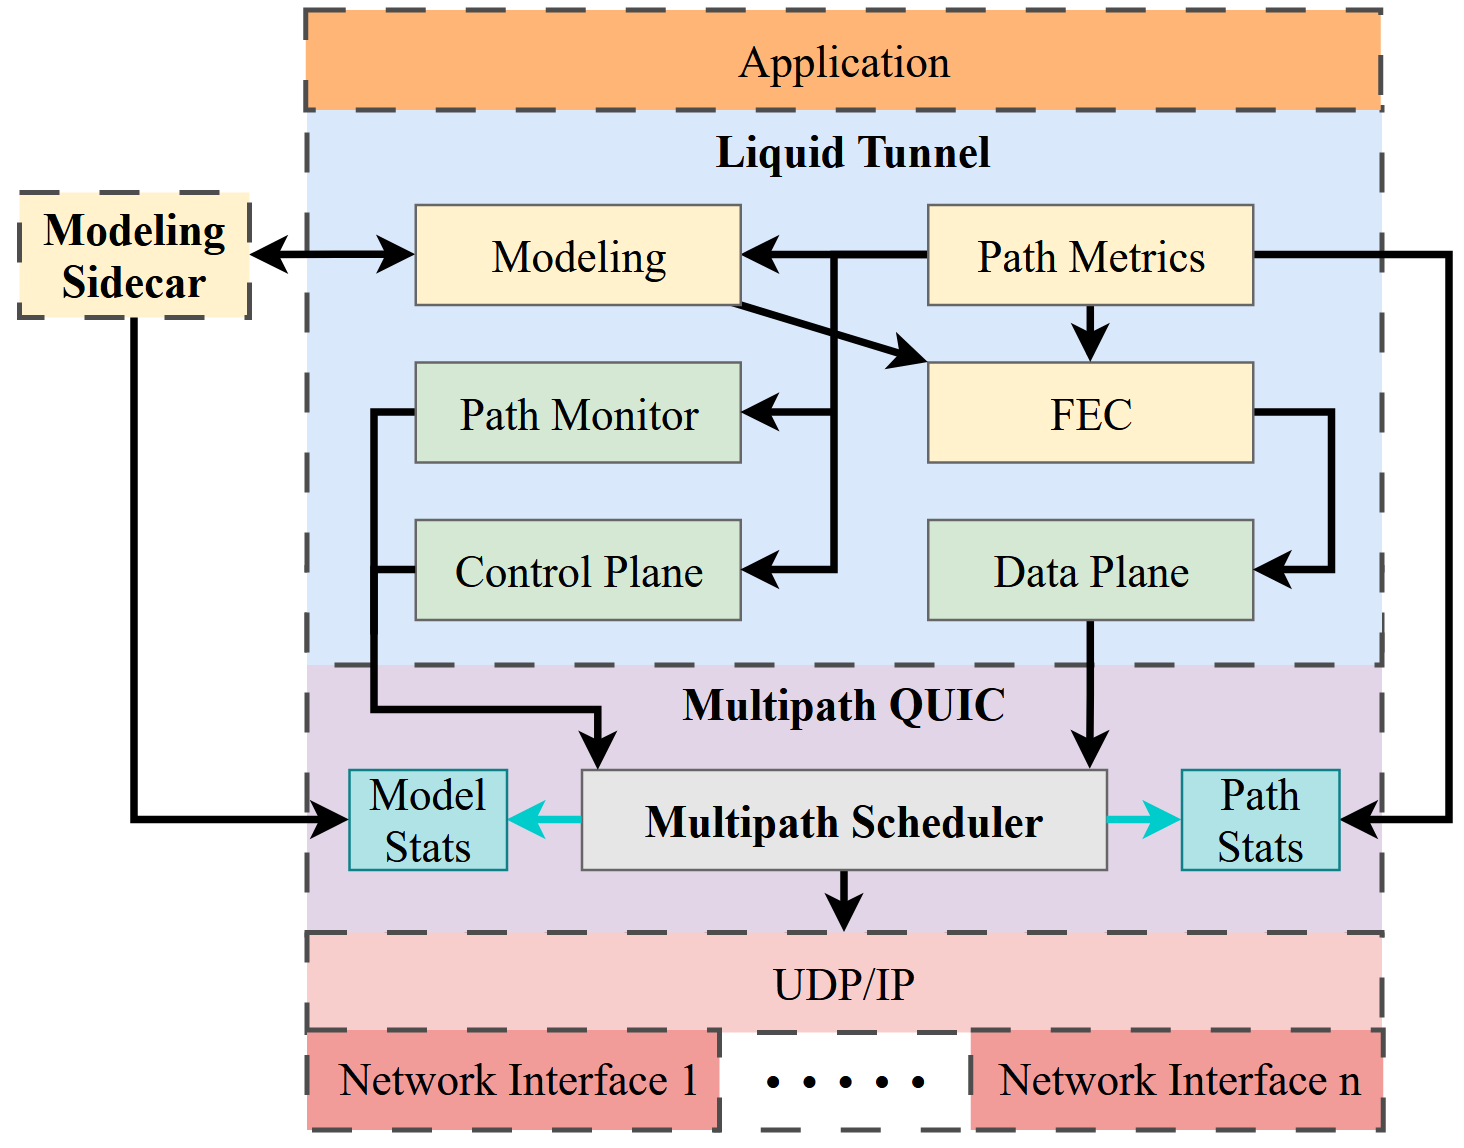
\includegraphics[width=\columnwidth]{images/tun_ip_stack.png}
    \caption{The IP stack architecture of the liquid tunnel.}
    \label{fig:ip_stack}
\end{figure}
% Path monitor
% QUIC Probes:
% Check if dead paths have recovered and probes stale paths for updates PathStats.

% Control plane
% QUIC Stream:
%   handshakes, keep alive to 
%   server, receives server's 
%   PathStats
% Feed PathStats into model.

% Data plane 
%   Datagrams:
%   send data into MPQUIC 
%   for scheduling 




% With multipath support, a single logical QUIC connection can utilize multiple network paths simultaneously. Each path maintains path-specific network state, while the scheduler determines the path over which each packet is transmitted. This decision is particularly important in heterogeneous networks because selecting the path with the lowest currently measured RTT does not necessarily result in the lowest packet-delivery time. A path that currently appears favorable may experience degradation shortly after transmission due to congestion, radio variation, satellite handover, or network reconfiguration.

\subsubsection{Network Configuration}
\label{subsubsec:network_configuration}

Our satellite-terrestrial integrated network is deployed using the ARA Wireless Living Lab \cite{ISLAM2025111188}. The real-world deployment is showcased in Fig. \eqref{fig:stin_setup}, where our client is deployed at an ARA user equipment unit located at a rural farm field in Ames, IA. Here, our PC connects to the Starlink UT and 5G radio using two separate physical interfaces. Here, the paths diverge over their respective wireless hops, where the Starlink traffic enters Starlink's LEO satellite network via the connected UT and exits their network after hopping from the UT to a satellite, then from the satellite to a ground station, and finally from the ground station to a point of presence (PoP) where it can access the Internet. In our case, the UT we use is associated with Starlink's Kansas City, MO PoP. Also at the UE, the 5G network takes its wireless hop to its associated base station, where it then routes to its 5G core before being able to access the Internet. In our deployment, this all occurs in Ames, IA. 

\begin{figure*}[!htbp]
    \centering
    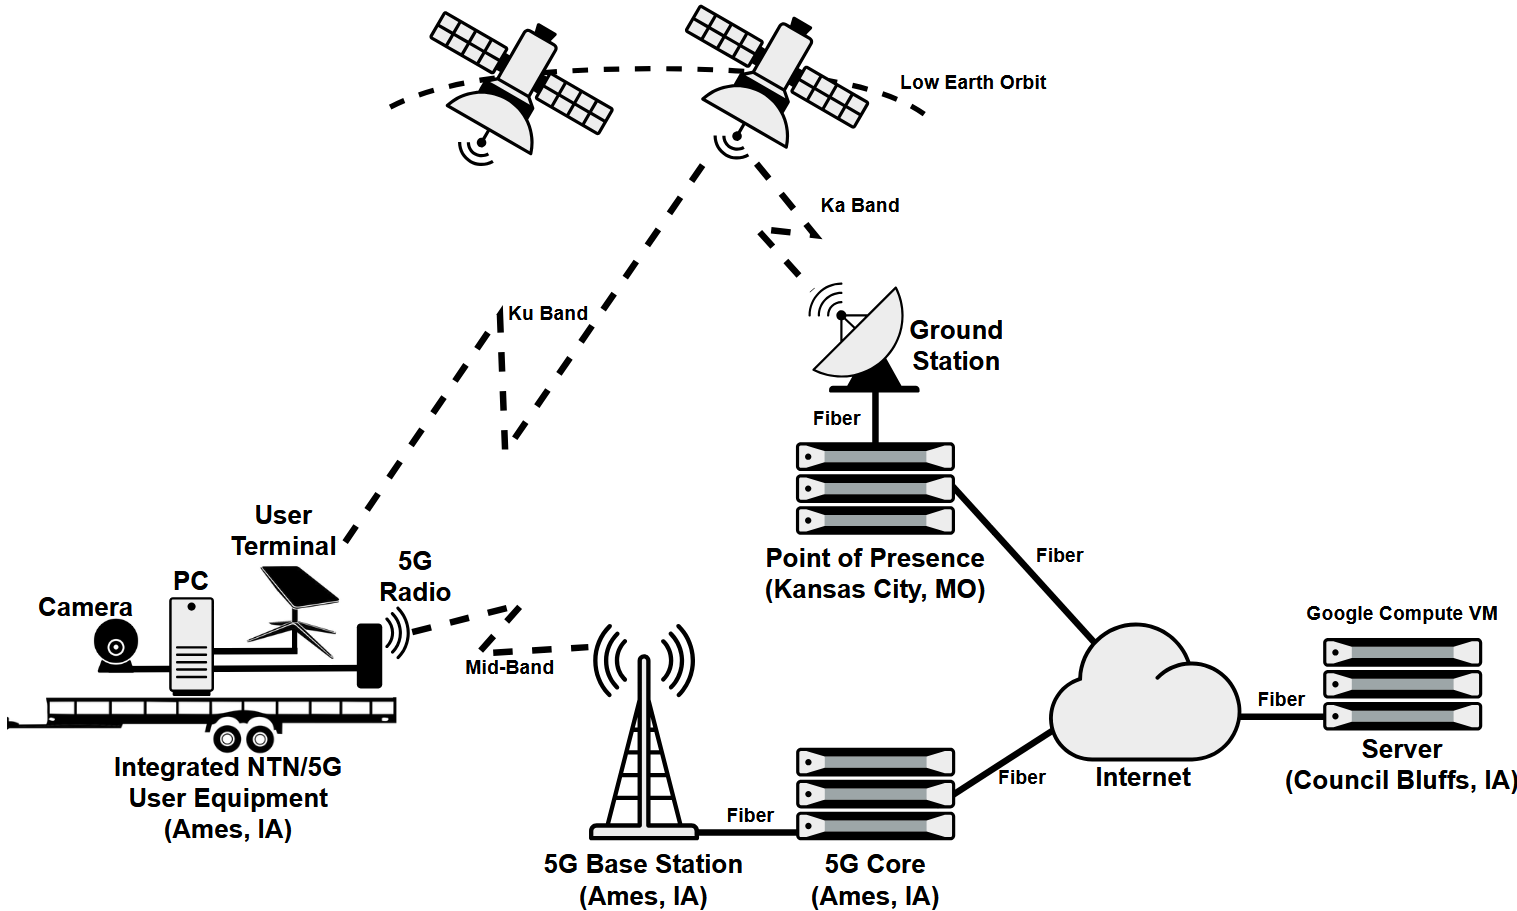
\includegraphics[width=0.6\textwidth]{images/real_world_setup.png}
    \caption{The real-world deployment setup of the STIN.}
    \label{fig:stin_setup}
\end{figure*}

The network configuration for our multipath deployment is a many-to-one connection (as required by MPQUIC). The client, which has multiple network interfaces, represents the many; the server must therefore have a singular address which all client IPs can communicate with. This is showcased in Fig. \eqref{fig:net_conf} with the client's two physical layer interfaces going to the singular server IP. 

This many-to-one connection is hidden from the client application's view. From its perspective, it will only use the singular IP assigned to the virtual tunnel interface.

The data flow is as follows:
\begin{enumerate}
    \item The server tunnel application is initialized. It creates a virtual tunnel interface and assigns it an IP, in this example, 10.0.0.1/24. The server then listens on 0.0.0.0:4433 for incoming requests from a client.
    \item The client tunnel application is initialized. It selects an initial physical network interface, in this case 10.189.55.160, and sends a QUIC handshake to the server's public IP, 136.64.133.110, using the selected physical interface.
    \item Upon successful completion of the handshake, the server selects an IP from its client tunnel IP pool, in this case 10.0.0.2/24, and assigns it to the client. It then communicates this address to the client.
    \item As the client receives the assigned address, it establishes its virtual tunnel interface using 10.0.0.2.
    \item With the QUIC handshake complete, the connection is identified by a Connection ID (CID), while each individual path remains associated with its own IP/port 4-tuple. The CID allows the connection to persist independently of the underlying network path. The connection then probes for additional paths for the multipath connection; in this case, 192.168.1.241 is probed and becomes available for use by the MPQUIC connection.
    \item Now that the MPQUIC connection is fully established and the tunnel is operational on both sides, the client application can begin transmitting data.
    \item The client application transmits its data to the server's tunnel IP, 10.0.0.1. The data enters the client's virtual tunnel interface at 10.0.0.2 and is forwarded through the liquid tunnel over the available MPQUIC paths to the server.
\end{enumerate}

This network configuration enables controlled comparison between single-path and multipath operation. Application traffic can be restricted to an individual path to establish terrestrial-only and satellite-only baselines, or both paths can be enabled simultaneously to evaluate multipath scheduling. The latter configuration provides the basis for comparing conventional reactive scheduling against the proposed prediction-aware approach.

\begin{figure*}
    \centering
    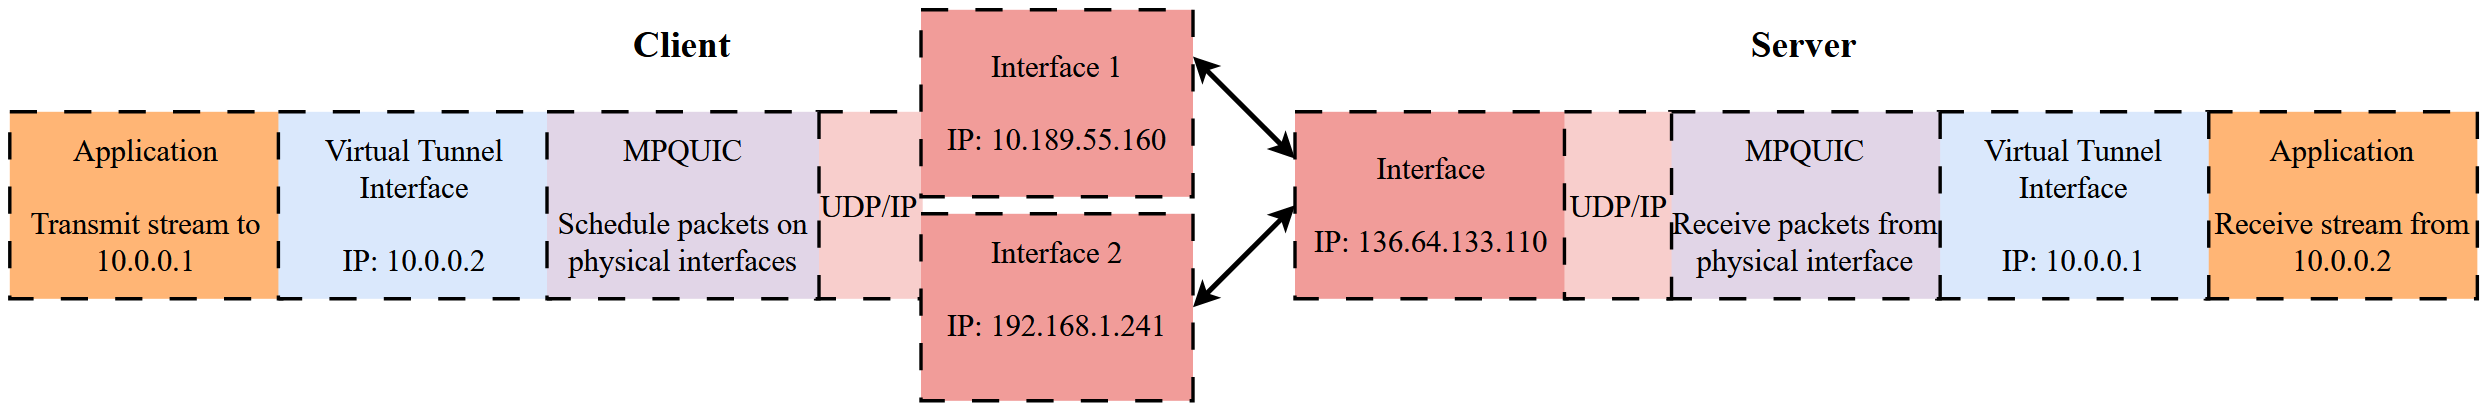
\includegraphics[width=\textwidth]{images/tun_network.png}
    \caption{The network configuration for the liquid tunnel as well as the traffic flow for a video stream from client to server.}
    \label{fig:net_conf}
\end{figure*}

% The Liquid Tunnel testbed is configured so that the communicating endpoints have access to multiple independent network interfaces representing heterogeneous end-to-end paths. The terrestrial interface is connected through the ARA 5G network, while the satellite interface is connected through Starlink's LEO satellite UT. Each interface is assigned to a distinct path within the multipath connection, allowing packets belonging to the same application session to be transmitted over different access technologies.

% The remote endpoint provides a common termination point for the multipath connection. This configuration is important because it allows differences in application performance to be attributed primarily to the access paths and scheduling decisions rather than to different application endpoints. Path-level measurements are collected continuously and associated with their corresponding interfaces, allowing the scheduler to maintain separate estimates of the operating conditions of the terrestrial and satellite links.

% \begin{figure*}[t]
% \centering
% \scalebox{0.80}{%
%     \input{images/tun_network}
% }
% \caption{The network configuration for the liquid tunnel, illustrating the MPQUIC-based multipath architecture between the client and server. The client application transmits traffic through a virtual tunnel interface, while MPQUIC schedules packets over multiple physical network interfaces. At the server, MPQUIC aggregates the packets received over the physical interface and forwards the reconstructed traffic through the virtual tunnel interface to the receiving application.}
% \label{fig:net_conf}
% \end{figure*}

\subsection{Model Integration}
\label{subsec:model_integration}

\subsubsection{Overview}

Each tunnel endpoint is responsible for predicting the behavior of its own network paths. Each side observes its local path telemetry and drives its own decisions from it. This self-directed design avoids any dependency on the peer's link conditions.
% however in our case it also means the server is unaware of the physical layer information that the client has.

Two system modules use these predictions within the tunnel: the forward error correction (FEC), which uses the predicted loss rate to configure redundancy, and the multipath packet scheduler, which uses the predictions to drive packet scheduling. These two modules are set up such that they can each use the same or different underlying models simultaneously, since sizing FEC redundancy and choosing a transmission path are logically independent decisions that happen to draw on overlapping input signals.

\subsubsection{Model Choices}

Three interchangeable models are currently available in the tunnel framework, selected independently for FEC and for scheduling:

\begin{itemize}
  \item \textbf{EMA (reactive)}: an exponentially-weighted moving average of instantaneous loss, computed directly from live path statistics. It reacts to a degradation only after it has occurred and offers no forward-looking estimate, so it is used for FEC only.
  \item \textbf{Kalman filter (predictive, sidecar-free)}: a per-path, per-metric constant-velocity Kalman filter tracking throughput, RTT, and loss. Because it carries both a value and a trend estimate, it can extrapolate a short horizon into the future rather than only smoothing the past. It requires no external process or physical-layer access, making it the natural choice on a side with no GPU for inference, or physical layer access for network information.
  \item \textbf{Sidecar (predictive, ML-based)}: a trained sequence model (per link provider) that additionally incorporates physical-layer and weather data unavailable to the tunnel. Interchangeable with any trained model that fits the feature structure.
\end{itemize}

\subsubsection{Inputs and Outputs}

All three models use the same base data: a rolling window of per-path throughput, RTT, and loss, derived from the QUIC layer's path telemetry. The sidecar model adds physical-layer data (signal strength, obstruction, satellite geometry) and local weather data, collected continuously by link-specific processes and merged into the feature vector for inference.

Regardless of source, a model produces two kinds of output. For FEC, the data-shard and parity-shard counts that dictate the redundancy to apply to outbound traffic. With multiple paths, redundancy is sized to protect against the worst currently active path. For scheduling, per-path predicted RTT, throughput, and packet loss are passed to the multipath scheduler, with a fallback to recent live data whenever a fresh prediction is unavailable for a given path.

\subsubsection{Sidecar Model Architecture and Communication}

The sidecar's predictive model is a sequence-to-sequence (seq2seq) recurrent network with attention, based on \cite{liu2025vivisecting}. It operates in a multi-input, multi-output configuration: it consumes the full input window of features dependent on if the path is 5G or Starlink, shown in Table \eqref{tab:model_features}, together with a learned cyclical time-of-day/day-of-week embedding, and produces a multi-step forecast over several target metrics simultaneously. The encoder is a two-layer gated recurrent unit (GRU) that compresses the input window into a sequence of hidden states. The decoder is a second GRU that generates the forecast autoregressively, one horizon step at a time; at each step it attends over the full encoder output using additive (Bahdanau) attention to focus on the most relevant portions of the input history, conditions on its own previous step's prediction, and projects the resulting hidden state to each target quantity through an independent output head. During training the decoder is exposed to true past values some fraction of the time (teacher forcing, annealed toward zero over training) to stabilize early learning while still training the model to rely on its own predictions at inference time, when no ground truth is available.

\begin{table}[!htbp]
    \centering
    \caption{Features used by the prediction model.}
    \label{tab:model_features}
    \begin{tabular}{|l||l|}
        \hline
        \textbf{Category} & \textbf{Feature} \\
        \hline
        \hline
        \multirow{3}{*}{Application}
            & Throughput \\
            & Packet loss \\
            & RTT \\
        \hline
        \multirow{3}{*}{Weather}
            & Weather humidity \\
            & Weather pressure \\
            & Weather rain rate \\
        \hline
        \multirow{3}{*}{5G}
            & RSRP \\
            & RSRQ \\
            & SINR \\
        \hline
        \multirow{10}{*}{Satellite}
            & Dish PoP latency \\
            & Satellite distance \\
            & Elevation degree \\
            & Azimuth degree \\
            & Dish obstruction fraction \\
            & Dish boresight azimuth degree \\
            & Dish boresight elevation degree \\
            & Is satellite DTC (0/1) \\
            & Satellite handoff occur (0/1) \\
            & Time since reconfiguration (0-15) \\
        \hline
    \end{tabular}
\end{table}

The sidecar model runs as a separate Python application, since its physical-layer and weather data collection is continuous and independent of any single tunnel connection's lifetime, and since the trained model itself is implemented and served outside the tunnel's own runtime. The tunnel process and the sidecar communicate over a local Unix domain socket, using a minimal length-prefixed JSON protocol: on each polling interval, the tunnel sends the current path window (throughput, RTT, loss samples) tagged with a link provider and path identifier, and the sidecar responds with a predicted horizon for the same three quantities, already denormalized into real units. If the sidecar is unreachable, times out, or has not yet accumulated a full window of physical-layer data, the request is treated as a missed prediction for that path rather than an error, and the FEC fusion will proceed over whatever paths did respond while the scheduler falls back to live telemetry for the affected paths.

% The central objective of integrating the temporal prediction models with the liquid tunnel is to provide the packet scheduler with short-term knowledge of future path conditions. The modeling framework described in this work generates forecasts of RTT, throughput, and packet loss from recent network observations and available cross-layer information. These predictions can be periodically supplied to the multipath scheduler and incorporated into its path-selection decisions.

% The integration follows a measurement--prediction--scheduling loop. First, path-specific measurements are collected from the available satellite and terrestrial interfaces. A sliding window of these measurements, together with the corresponding network-specific features, forms the input to the prediction model. The trained model then produces forecasts over the configured prediction horizon. Finally, the predicted QoS values are supplied to the Liquid Tunnel scheduler, which uses them together with the current path state to determine how subsequent packets should be distributed.

% For the Seq2Seq-GRU model considered in this work, an input window of recent observations is used to simultaneously forecast RTT, throughput, and packet loss over a 15-second horizon. The experimental results, however, indicate that the useful prediction horizon is metric-dependent. RTT retains meaningful temporal predictability over longer intervals for several of the evaluated links, whereas throughput and packet-loss prediction accuracy decreases substantially after approximately 3--5 seconds. Consequently, the scheduler should not necessarily treat all predicted quantities or forecast horizons equally. Near-term forecasts can be assigned greater importance, while longer-horizon predictions may primarily be used to identify persistent trends or anticipated path degradation.

% The prediction output can be represented by a path cost that combines the QoS requirements of the application. For example, a general prediction-aware path metric may be expressed as
% \begin{equation}
% C_p(t+\tau)
% =
% w_r \hat{r}*{p}(t+\tau)
% +
% w_j \hat{j}*{p}(t+\tau)
% +
% w_{\ell}\hat{\ell}_{p}(t+\tau),
% \label{eq:predicted_path_cost}
% \end{equation}
% where $w_r$, $w_j$, and $w*{\ell}$ are application-dependent weights associated with RTT, throughput, and packet loss, respectively. The scheduler can favor the path with the lowest expected cost or use the costs to determine traffic-splitting weights across multiple paths. For real-time applications, the weights can be selected to strongly penalize latency, throughput, and packet-loss conditions that would degrade application QoE.

An important benefit of this architecture is that the prediction model does not directly control packet transmission. Instead, it provides additional information to the scheduling layer, while Liquid Tunnel retains responsibility for the actual path-selection decision. This separation allows different prediction models and scheduling policies to be evaluated independently and makes it possible to fall back to conventional measurement-based scheduling when predictions are unavailable or insufficiently reliable.

Ultimately, the integration of Liquid Tunnel and the temporal prediction framework enables a transition from reactive to proactive multipath communication. Rather than waiting for a path degradation event to become visible through increased RTT or packet loss, the scheduler can anticipate the degradation and redirect traffic beforehand. The evaluation of this prediction-aware scheduling mechanism over integrated 5G and LEO satellite paths, particularly for latency-sensitive real-time applications, constitutes the next stage of this work.

\section{QoE-Predictive Scheduler}
\label{sec:qoe_scheduler}

We implement an initial intelligent packet scheduling algorithm \textit{QoE-Predictive Scheduler}. It treats each active path $i$ as a single-server queue and estimates the time a newly scheduled packet would take to arrive if sent on that path. Let $F_i$ be the bytes currently in flight on path $i$, $B_i$ its throughput estimate (predicted if fresh, else the live delivery rate), $s$ the packet size, and $\hat{R}_i$ the predicted RTT. We define predicted arrival time as:

\begin{equation}
    \hat{T}_i^{\text{arr}} \;=\; \underbrace{\frac{F_i}{B_i}}_{\text{drain}}
    \;+\; \underbrace{\frac{s}{B_i}}_{\text{serialization}}
    \;+\; \underbrace{\frac{\hat{R}_i}{2}}_{\text{one-way latency}}
    \label{eq:arrival}
\end{equation}
This is the scheduler's estimate of "if I send this packet on path $i$ right now, when will it get to the other side?"

Two additional terms distinguish QoE from a plain arrival-time minimizer. First, a \emph{reordering penalty}: let $H$ be the high-water mark, the latest predicted arrival time among already-dispatched packets,
% with a smaller sequence number
and $\tau$ a tolerance. $\tau$, the reorder tolerance, may be hand picked or derived from RTT variation.
% "how much lateness relative to the other paths is acceptable before I start penalizing it" knob
A candidate path violates the reordering penalty when:

\begin{equation}
    V_i \;=\; \max\!\big(0,\; H - \hat{T}_i^{\text{arr}} - \tau \big)
\end{equation}

Second, a congestion term $U_i = F_i / C_i$ (in-flight bytes over congestion window, capped at 1) and a loss term $L_i = \max_{k \le w} \hat{\ell}_{i,k}$, the worst predicted loss over the next $w$ forecast steps. The per-path cost is a weighted sum:

\begin{equation}
    J_i \;=\; w_R\, V_i \;+\; w_U\, U_i \;+\; w_L\, L_i
    \label{eq:cost}
\end{equation}

and the scheduler selects

\begin{equation}
    i^{*} \;=\; \operatorname*{arg\,min}_{i \,\in\, \mathcal{P}_{\text{on-time}}} J_i,
    \qquad
    \mathcal{P}_{\text{on-time}} \;=\; \{\, i : \hat{T}_i^{\text{arr}} \le d \,\}
    \label{eq:decision}
\end{equation}

where $d$ is the packet's deadline. $J_i$ is the total cost for a path and is the single number the scheduler uses to rank paths that already meet the deadline. $\mathcal{P}_{\text{on-time}}$ is the on-time candidate set, which is the subset of active paths that pass the hard deadline test.
If $\mathcal{P}_{\text{on-time}} = \emptyset$, the packet is dropped (or sent on the least-late path, depending on policy), rather than relaxing the deadline constraint.

\begin{algorithm}[h]
\caption{QoE-Predictive path selection}
\label{alg:qoe}
\begin{algorithmic}[1]
\Require active paths $\mathcal{P}$, packet deadline $d$, sequence number $\text{seq}$
\State $H \gets$ high-water mark of predicted arrivals for seq $< \text{seq}$
\ForAll{$i \in \mathcal{P}$}
    \State compute $\hat{T}_i^{\text{arr}}$ via Eq.~\eqref{eq:arrival}
    \If{$\hat{T}_i^{\text{arr}} \le d$}
        \State compute $J_i$ via Eq.~\eqref{eq:cost} and add $i$ to $\mathcal{P}_{\text{on-time}}$
    \EndIf
\EndFor
\If{$\mathcal{P}_{\text{on-time}} \ne \emptyset$}
    \State $i^{*} \gets \arg\min_i J_i$, subject to a hysteresis check against the current path
\Else
    \State \Return \textsc{Drop} (or least-late path, per policy)
\EndIf
\State record $\hat{T}_{i^{*}}^{\text{arr}}$ for future high-water-mark lookups
\State \Return path $i^{*}$
\end{algorithmic}
\end{algorithm}

Equation~\eqref{eq:arrival} is a queuing-theoretic estimate which models each path as a G/G/1-style server whose backlog ($F_i/B_i$) must drain before a new packet is served. Because it is recomputed from live and forecasted state every packet, the scheduler reacts to congestion and loss \emph{before} they show up in measured RTT. The deadline constraint in Eq.~\eqref{eq:decision} exists as tunneled, non-retransmitted traffic gets no benefit from a "fast but late" path; a late packet is worthless, so excluding it outright (rather than merely penalizing it) matches the traffic's actual utility function. The reordering term $V_i$ exists because path quality alone is insufficient for real-time delivery: a path can have an excellent predicted arrival time and still be the wrong choice if it would deliver \emph{out of order} relative to packets already in flight, since downstream consumers of real-time streams are typically as sensitive to jitter/reordering as to raw latency. Finally, hysteresis on the arg min prevents the scheduler from rapid path switching due to small, noisy score differences between paths, which would otherwise reintroduce the very reordering problem $V_i$ is meant to suppress.

\section{Experimentation Setup}
\label{sec:experimentation}


\subsection{Platform, Hardware, and Software}
\subsubsection{Platform \& Hardware}
To demonstrate the effectiveness of the liquid tunnel, we deployed and evaluated it in the ARA Wireless Living Lab~\cite{islam_design_2024}, an at-scale experimental testbed deployed in Central Iowa. ARA enables the research and development of rural-focused wireless technologies and a key feature of it is the availability of a deployed rural 5G testbed hosting multiple wireless backhaul and radio access network technologies deployed at various base stations (BSes) and User Equipments (UEs). Radio access network technologies are enabled at the UEs with the availability of multiple network interfaces operating at multiple frequency bands such as TV White Space (TVWS) (460--776 MHz), mid-band (3.4--3.6 GHz), mm-Wave (27.50--28.35 GHz), and NTN with Ku (12--18 GHz) and Ka (26.5--40 GHz) bands. 

For our experiments, we use an ARA trailer UE deployed on a rural farm multiple 5G UEs and our Starlink terminal, shown in Fig. \eqref{fig:trailer_ue}. We primarily use a COTS Quectel module operating in the mid-band Ericsson network offering up to 100\,Mbps UL and 600\,Mbps DL with a range of up to 4\,km for our terrestrial 5G, and for our NTN we use a Starlink Mini offering up to 35\,Mbps UL and 260\,Mbps DL. In reality at our deployment location, we average a maximum of 110\,Mbps UL/320\,Mbps DL for Quectel and 40\,Mbps UL/90\,Mbps DL for Starlink.

\begin{figure}
    \centering
    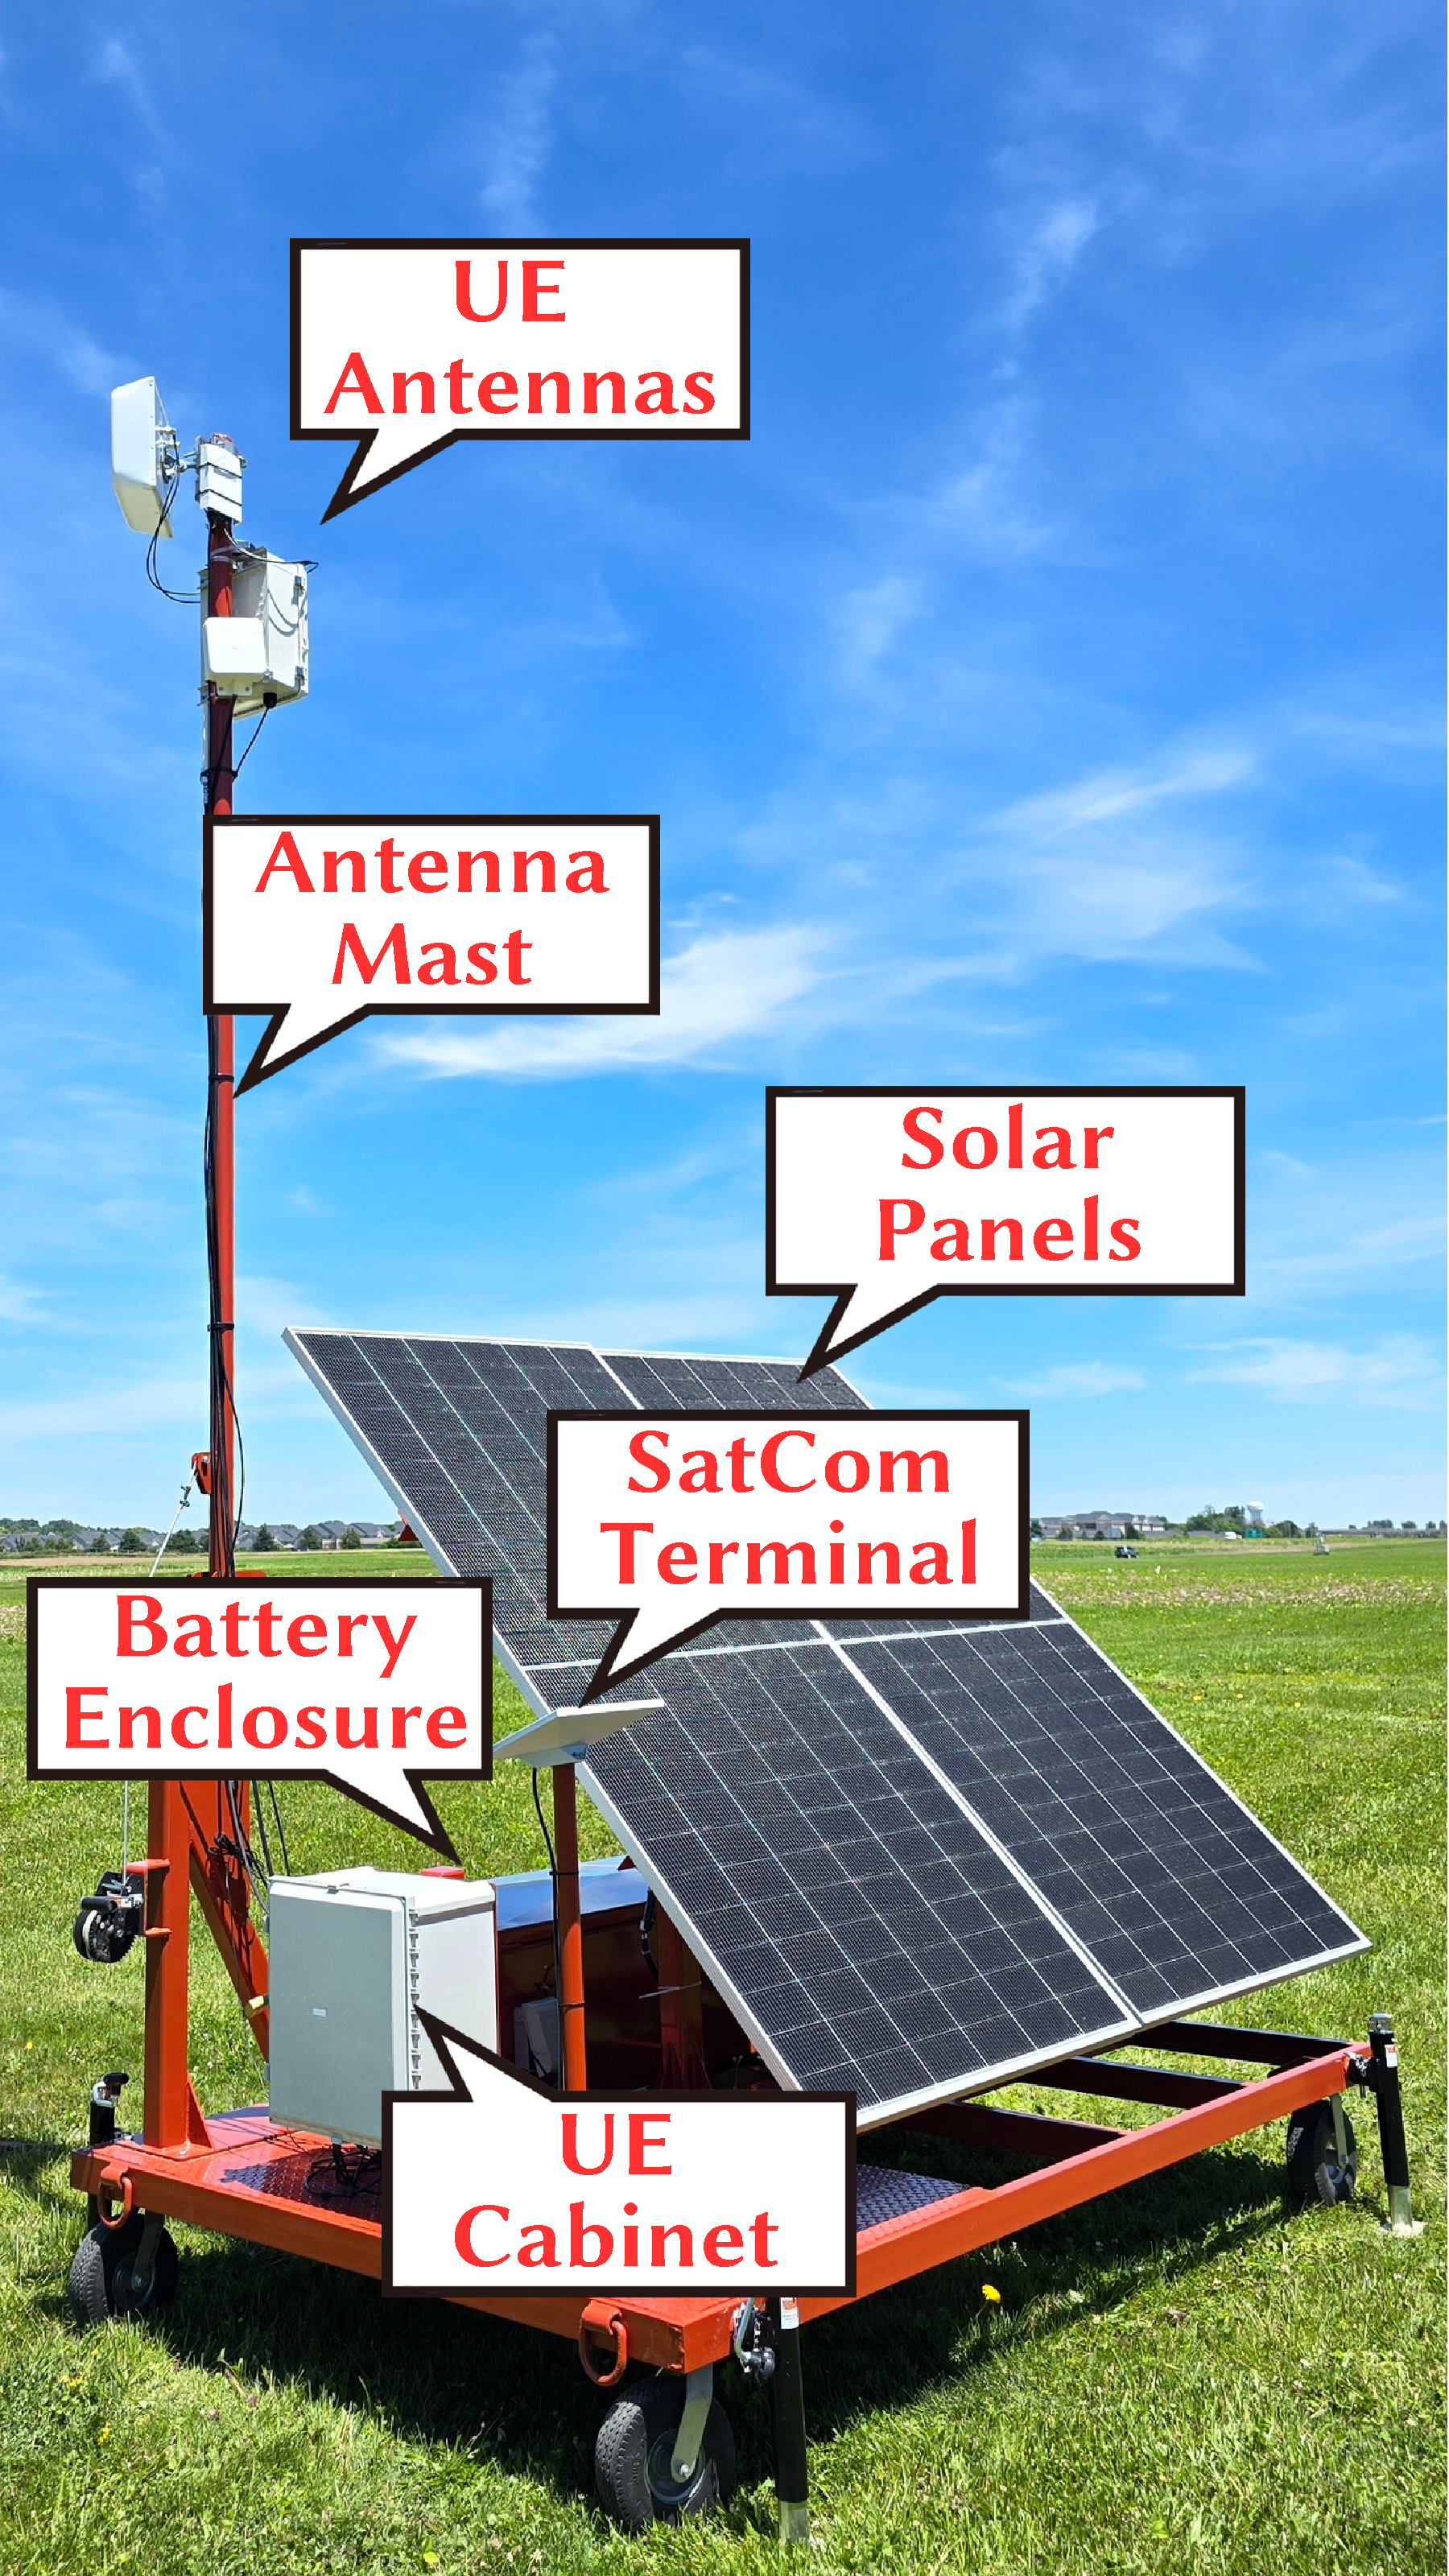
\includegraphics[width=0.7\columnwidth]{images/trailer_ue.pdf}
    \caption{The real-world STIN UE.}
    \label{fig:trailer_ue}
\end{figure}

Other than the Starlink Mini and Quectel COTS UE, we also have our computing hardware. For the UE computer, we use ARA's system, which runs Ubuntu 22.04.5 LTS on a Linux 5.15.0-186-generic kernel and has an Intel Xeon D-1736NT CPU and 32\,GB RAM.

For our server, we use a Google Compute VM located in Council Bluffs, IA. Specifically, we use an e2-standard-2 general-purpose VM with 2 vCPUs and 8 GB of RAM, which is optimized for balanced CPU and memory workloads.

\subsubsection{Software}
For our software, we use an MPQUIC implementation written in Rust and based on Cloudflare's Quiche QUIC repository\footnote{\url{https://github.com/qdeconinck/quiche}}. We specifically use a previous pull request of this repository that includes multipath Quiche with Tokio Quiche support\footnote{\url{https://github.com/bastienvty/quiche/tree/mpquic-in-tokio}}. Tokio for Rust is an async runtime that provides an event loop, scheduling, and non-blocking I/O for writing high-concurrency network and task code.

For our tunnel's modeling sidecar, we use Python and PyTorch. The sidecar allows for swapping the models as long as they share the same input features and outputs. The sidecar also handles the collection of our weather data using ARA's weather API and Python library, as well as the Quectel physical layer data. It also makes gRPC calls to the Starlink UT's API to collect the Starlink data.

For our application, we develop a GStreamer RTP/H.264-over-UDP sender/receiver video-streaming application. This allows us to transmit a real-time video stream over UDP using RTP to our server from our client. The server is able to capture our application metrics such as packet arrival time, packet dispersion, packet loss, packet reordering, received bitrate, packet count, frame arrival, inter-frame arrival (IFA), FPS, and dropped frames.

\section{Measurement Results}
\label{sec:eval}

To evaluate our transport, path model, and intelligent scheduling algorithm, we transmit a 4K 30 FPS video stream at 45\,Mbps from our client in the field to our Google Compute VM. From the client/UE perspective, we are therefore focused on the UL paths of Quectel and Starlink. We focus on analyzing the application metrics to see how the path modeling and intelligent scheduling algorithm both benefit the application and increase the QoE.

We specifically compare single path performance against multipath with the default minimum RTT (minRTT) algorithm to confirm the liquid tunnel with multipath enhances QoE over single path. We then compare the multipath schedulers of minRTT, a predictive-minRTT algorithm using the path predictions, as well as the QoE-predictive scheduler. All measurements are conducted using the liquid tunnel; this includes the single-path network measurements which run as a single path liquid tunnel. \textbf{For this report, no FEC is utilized in the tunnel.}

We define the predictive-minRTT algorithm below:

For each active path $i$, let $\hat{R}_i$ and $\hat{B}_i$ denote the mean predicted RTT
and throughput over the forecast horizon, and $\hat{\ell}_i$ the mean predicted loss
(as a fraction). The path quality score is

\begin{equation}
    Q_i \;=\; \frac{\hat{R}_i}{\hat{B}_i} \,\big(1 + \hat{\ell}_i\big)^{2},
\end{equation}

and the scheduler selects

\begin{equation}
    i^{*} \;=\; \operatorname*{arg\,min}_i \, Q_i .
\end{equation}

If no fresh prediction exists for a path, $\hat{R}_i$ falls back to its live
$\text{RTT} + 2\cdot\text{RTT}_{VAR}$ and $\hat{B}_i, \hat{\ell}_i$ are omitted from the
score.

We further analyze the following metrics in our evaluation:
\begin{itemize}
    \item \textbf{FPS:} Average number of video frames decoded per second.
    \item \textbf{Packet Loss:} Percentage of transmitted packets that are not received.
    \item \textbf{Frame Loss:} Number of video frames lost or unable to be decoded per second.
    \item \textbf{Packet Dispersion:} Time interval between consecutive received packets, measured in $\mu$s.
    \item \textbf{Inter-Frame Arrival (IFA):} Time interval between consecutive received video frames, measured in ms.
    \item \textbf{Received Bitrate:} Rate of successfully received video data, measured in Mbps.
    \item \textbf{Total Packet Loss:} Total number of packets lost during the stream.
    \item \textbf{Total Frame Loss:} Total number of video frames lost during the stream.
\end{itemize}

To start, we confirm in Figs. \eqref{fig:fps_paths}, \eqref{fig:frame_loss_paths}, \eqref{fig:ifa_paths}, as well as Table \eqref{tab:video_performance}, that minRTT provides higher FPS and lower packet losses, frame losses, IFA times, and packet dispersion than both Starlink and Quectel. Furthermore, Quectel, with higher UL speeds and no frequent network configuration (such as Starlink experiences) performs better than Starlink. We also note that the sending bitrate for the video stream is a static (not adaptive) 45\,Mbps as mentioned earlier, so the erratic and unstable behavior Starlink showcases is not a surprise. We do however, confirm that multipath, even in such a heterogeneous environment as STIN, provides a higher QoE than single path.

\subsection{Path Modeling}

The path modeling itself is of key importance to this study. We compare the predictive-minRTT scheduler, which uses the path models, against the baseline minRTT scheduler. As shown in Fig. \eqref{fig:fps_schedulers} and the table, the predictive-minRTT and minRTT seem to perform very similarly when considering only FPS. However, when looking at the other application metrics we see that utilizing the path models helps the scheduler perform much better than the baseline minRTT. In Fig. \eqref{fig:frame_loss_schedulers}, predictive-minRTT has significantly less spikes in frame losses, which is also shown in Table \eqref{tab:video_performance} with $52\%$ less frames lost per second on average compared to minRTT, and over half as many less frames dropped overall. 

This showcases that utilizing path models with even a basic scheduler to be proactive is more beneficial than being solely reactive. 

\begin{figure}[!htbp]
    \centering

    \begin{subfigure}[b]{\columnwidth}
        \centering
        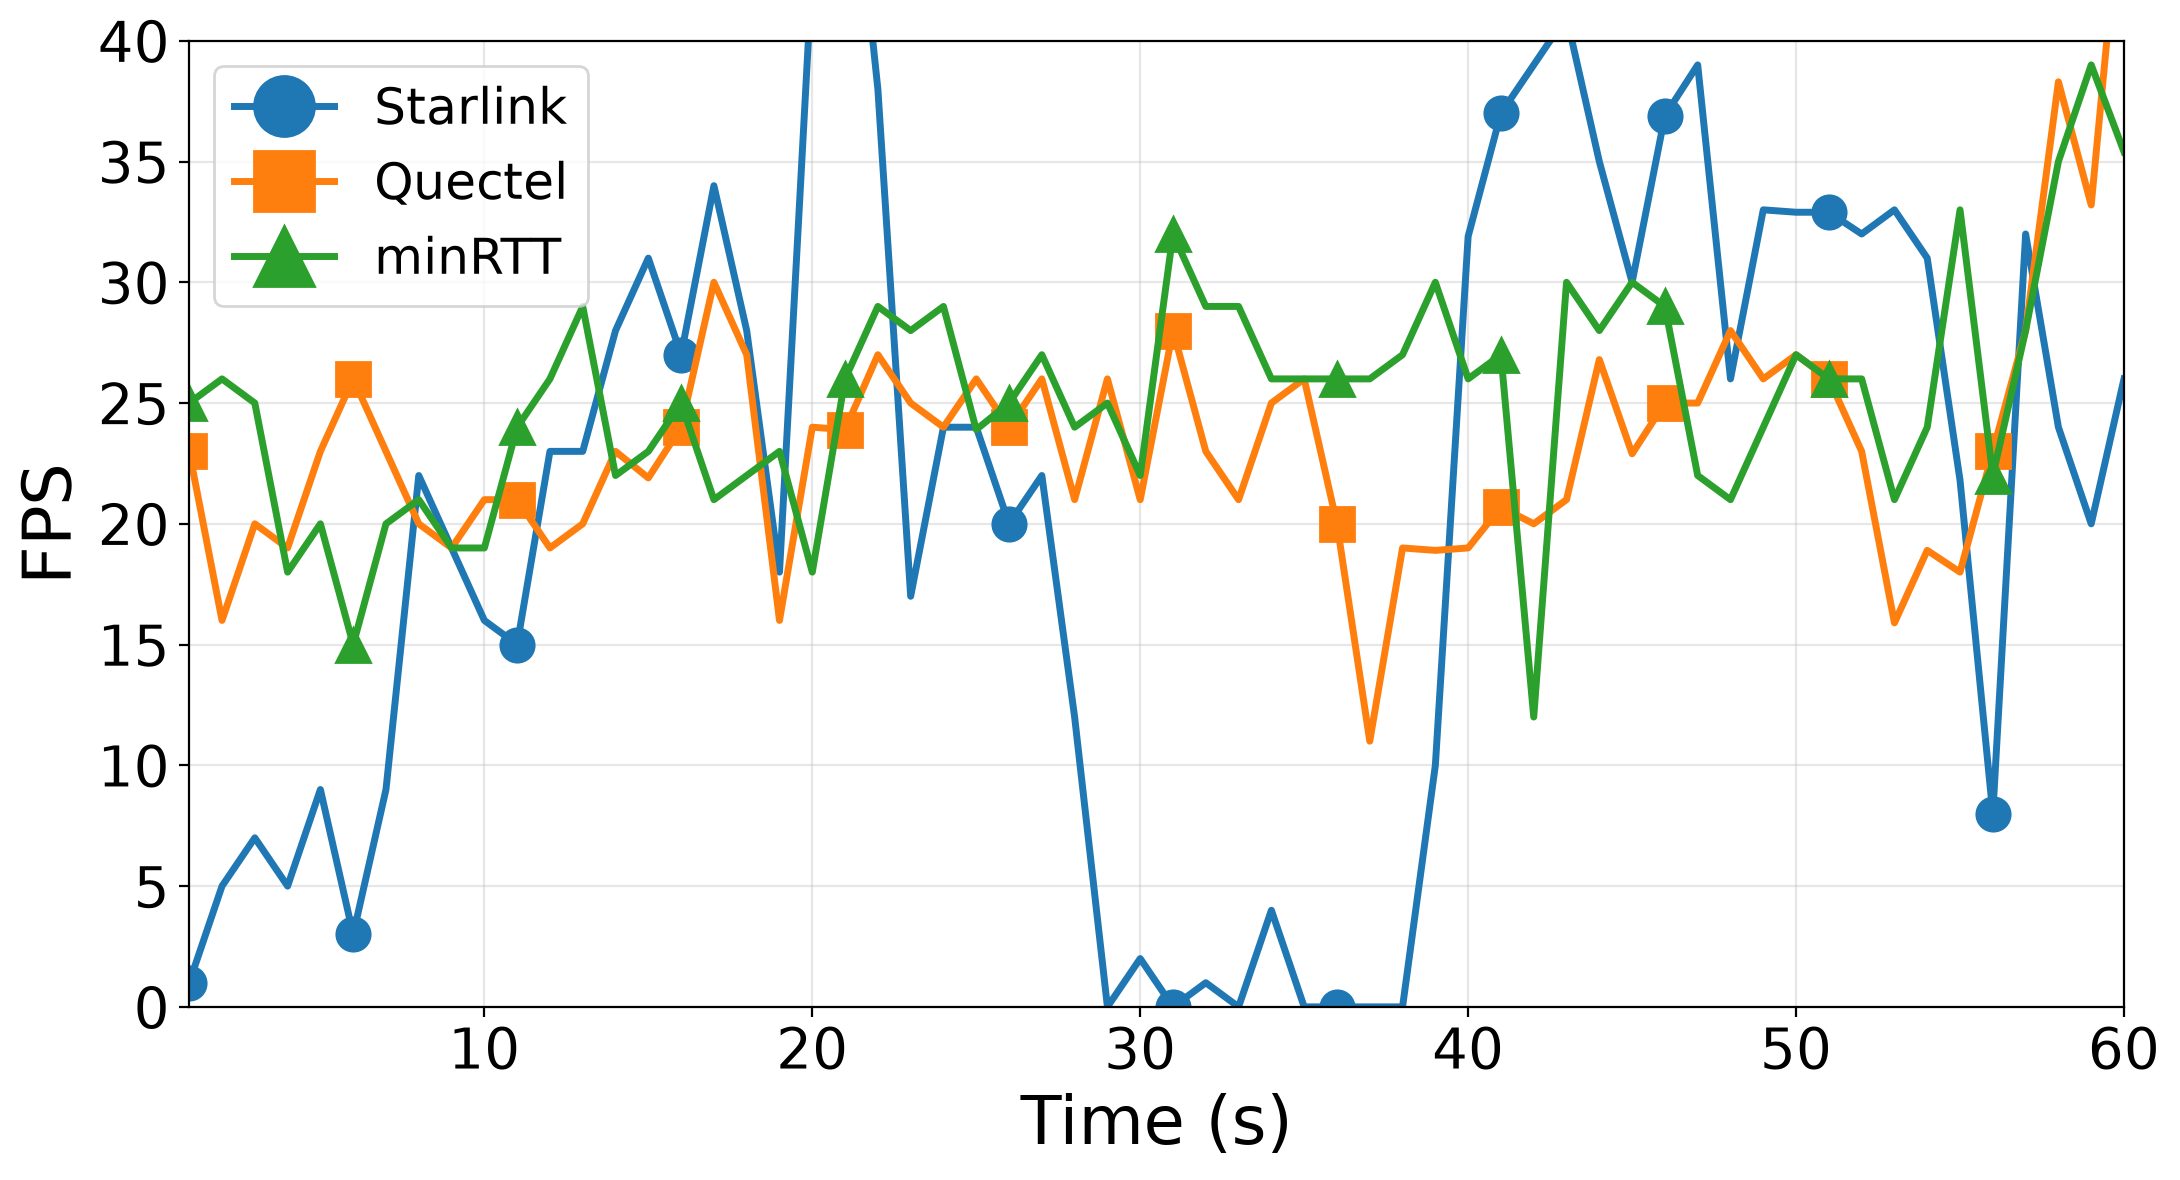
\includegraphics[width=\columnwidth]{images/fps_paths.png}
        \caption{Starlink, Quectel, and minRTT.}
        \label{fig:fps_paths}
    \end{subfigure}

    \vspace{0.5em}

    \begin{subfigure}[b]{\columnwidth}
        \centering
        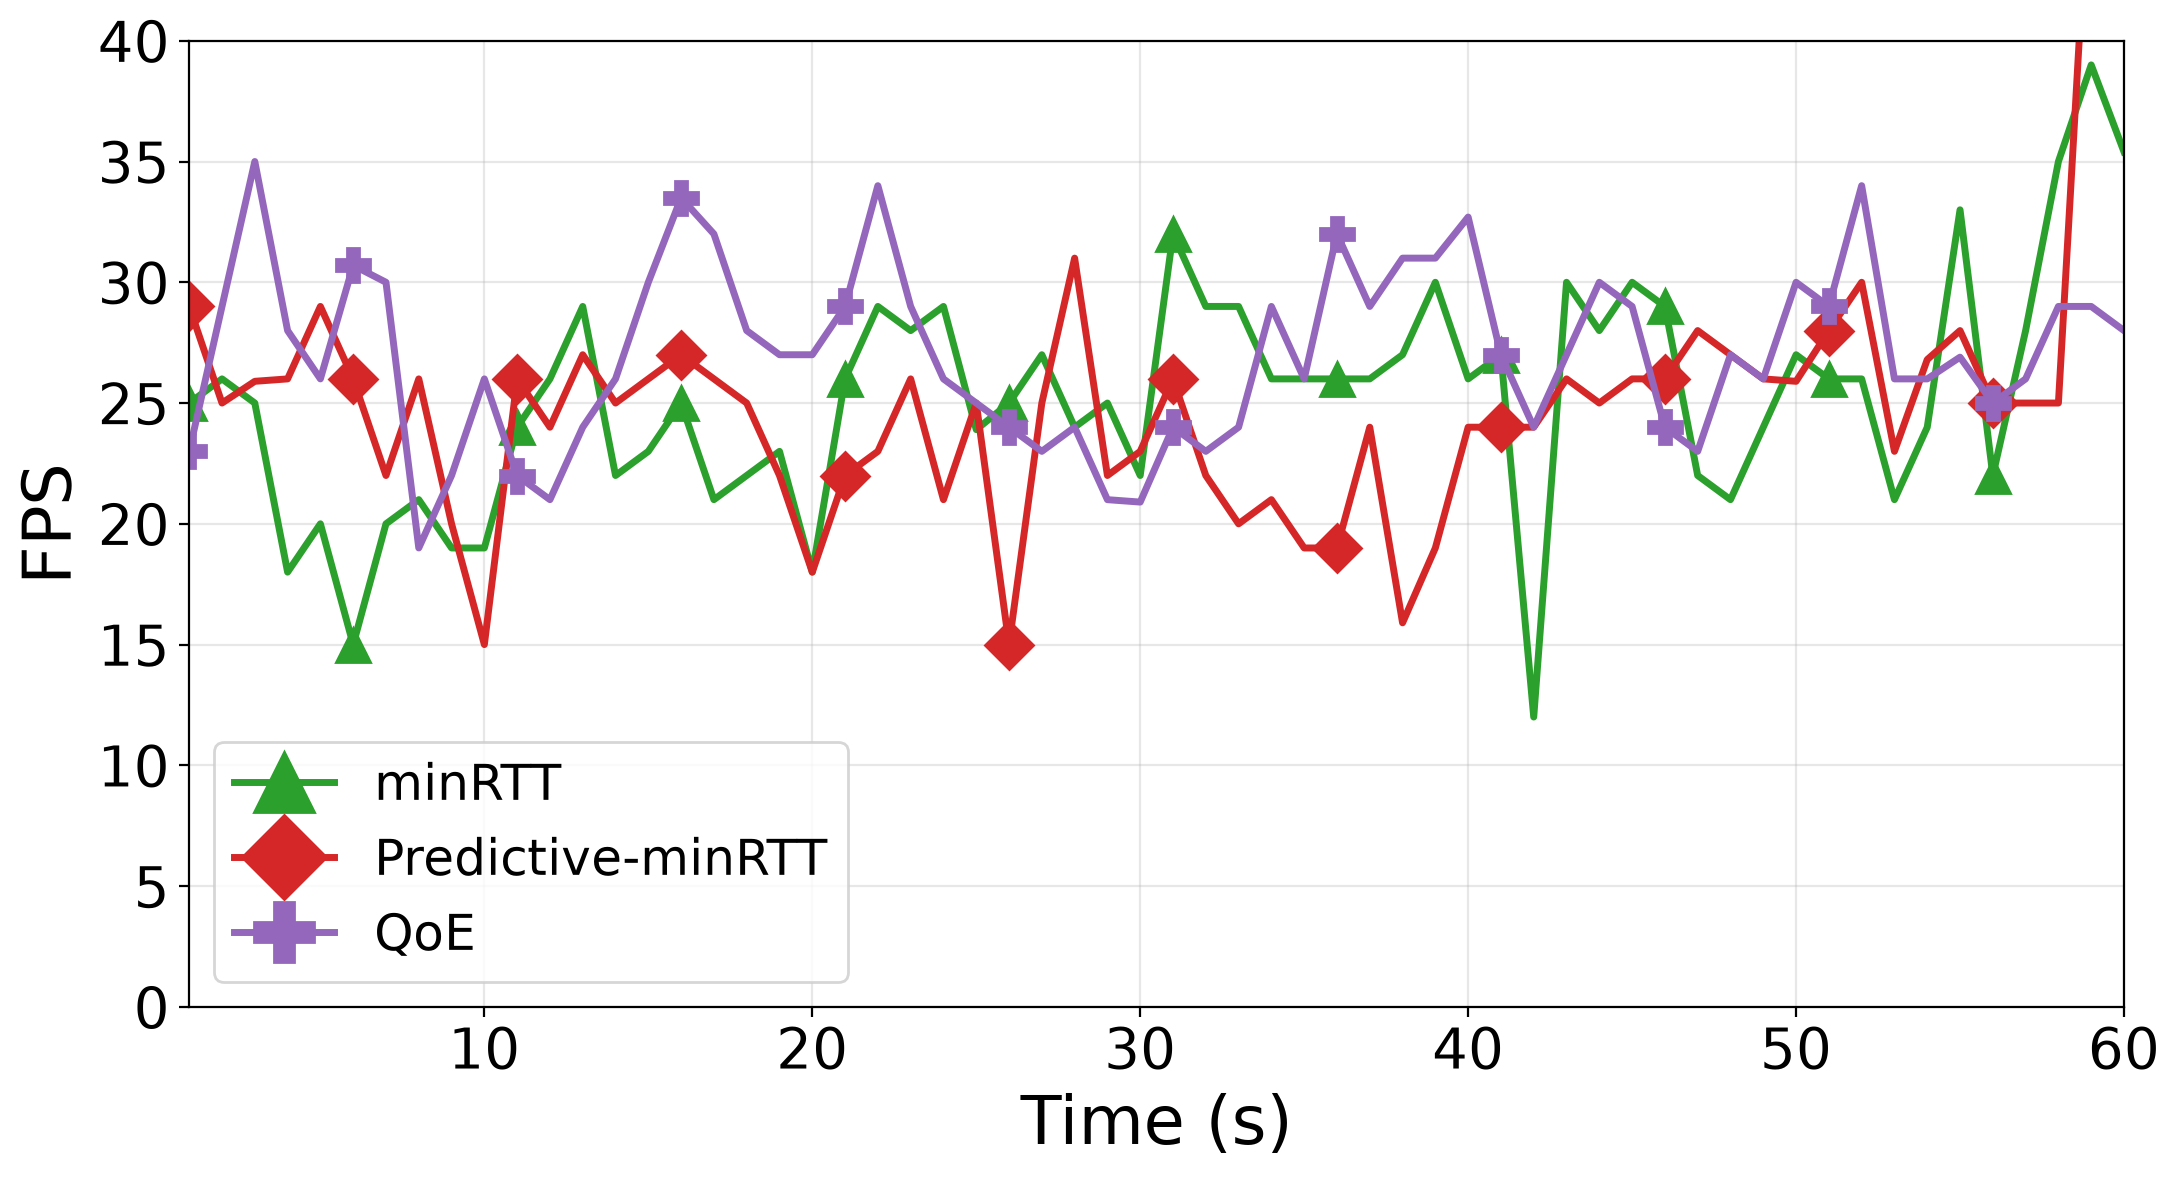
\includegraphics[width=\columnwidth]{images/fps_schedulers.png}
        \caption{Packet scheduling comparison.}
        \label{fig:fps_schedulers}
    \end{subfigure}

    \caption{Frame rate comparison across network paths and packet scheduling algorithms.}
    \label{fig:fps_comparison}
\end{figure}


\begin{figure}[!htbp]
    \centering

    \begin{subfigure}[b]{\columnwidth}
        \centering
        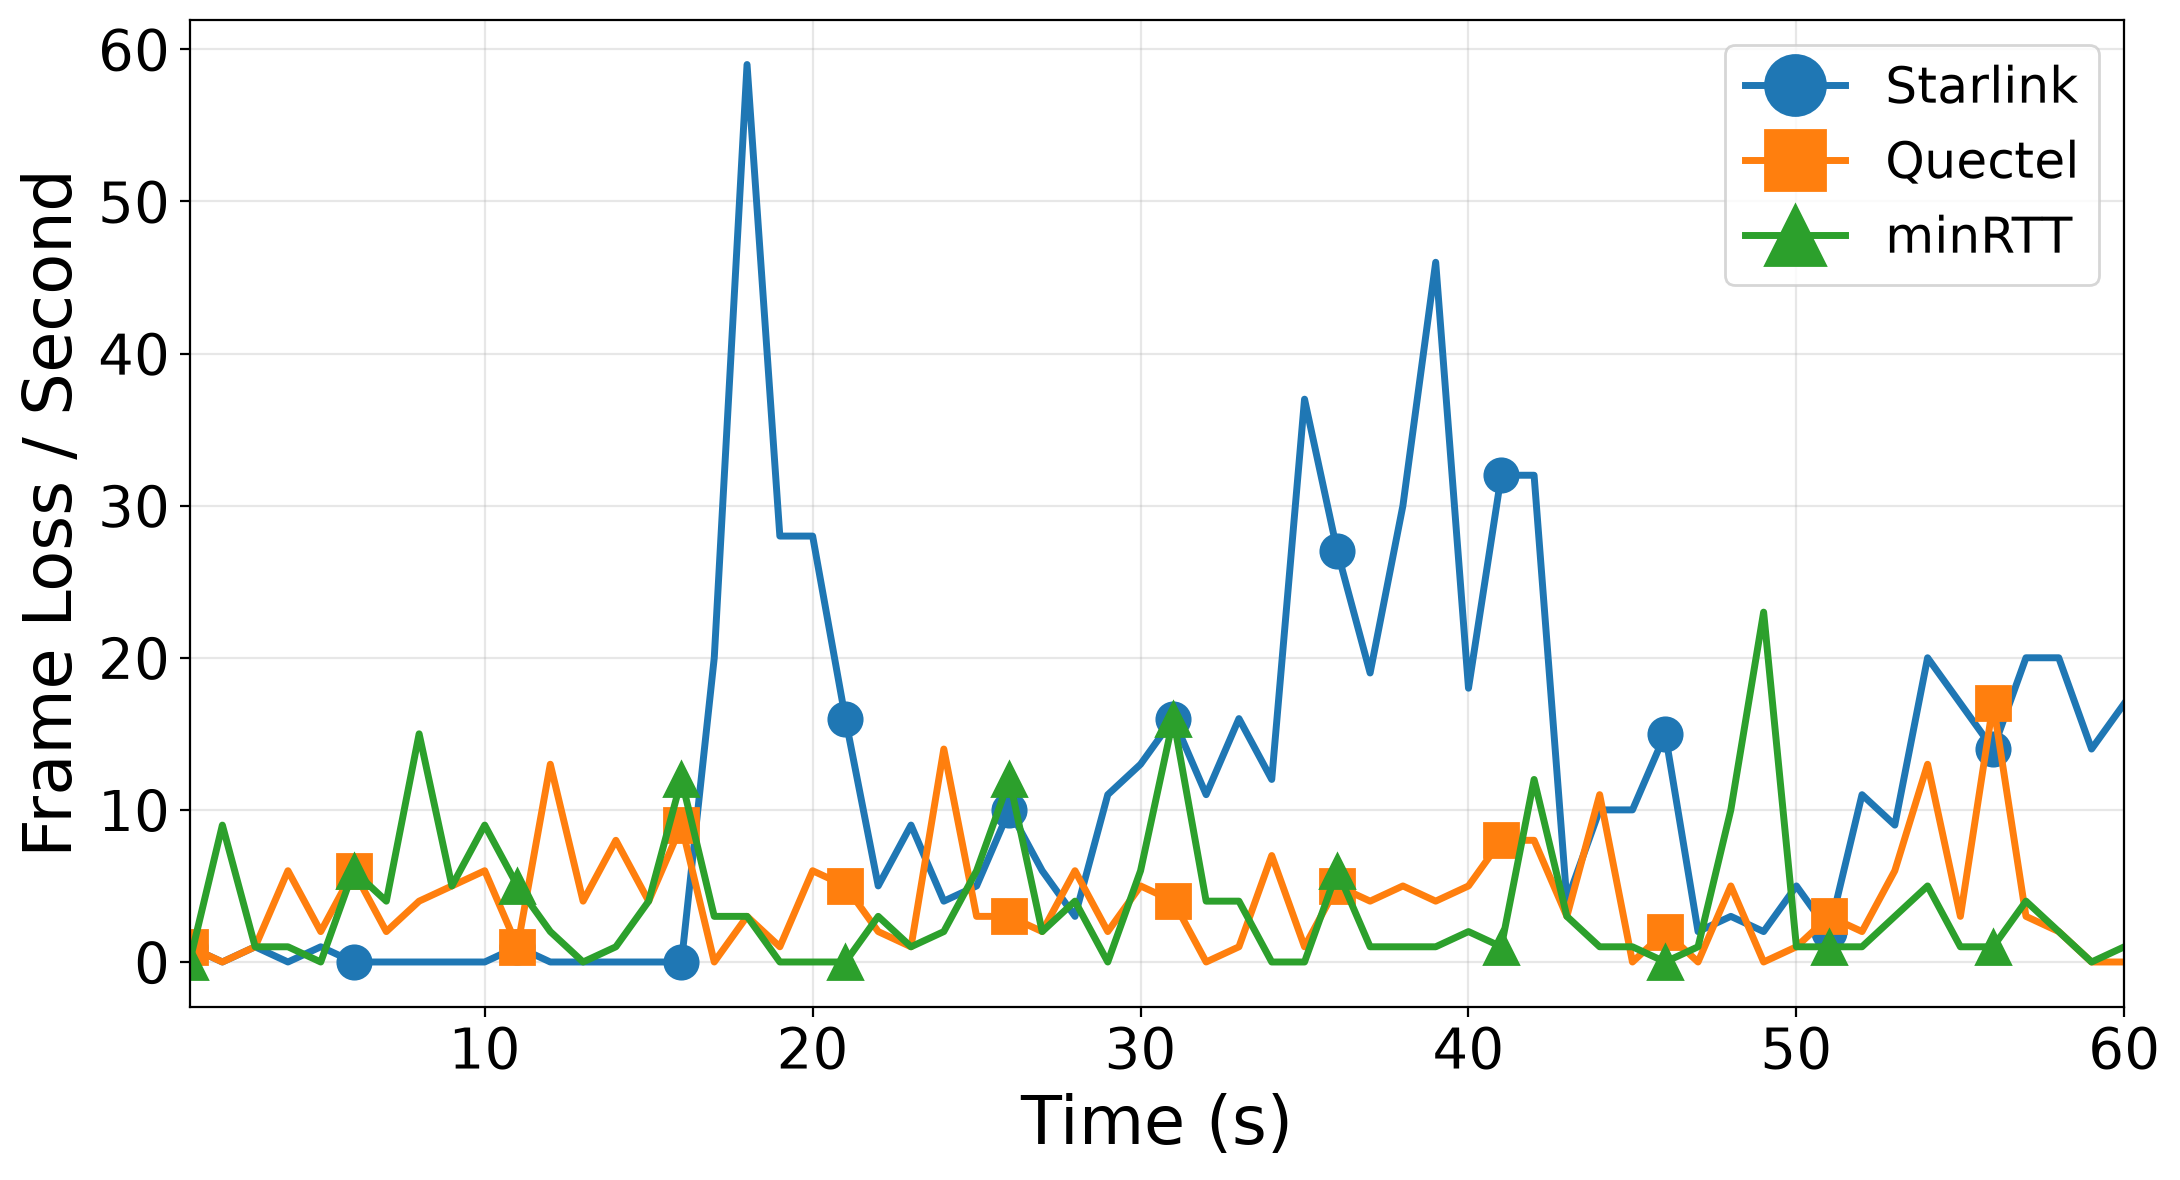
\includegraphics[width=\columnwidth]{images/frame_loss_paths.png}
        \caption{Starlink, Quectel, and minRTT.}
        \label{fig:frame_loss_paths}
    \end{subfigure}

    \vspace{0.5em}

    \begin{subfigure}[b]{\columnwidth}
        \centering
        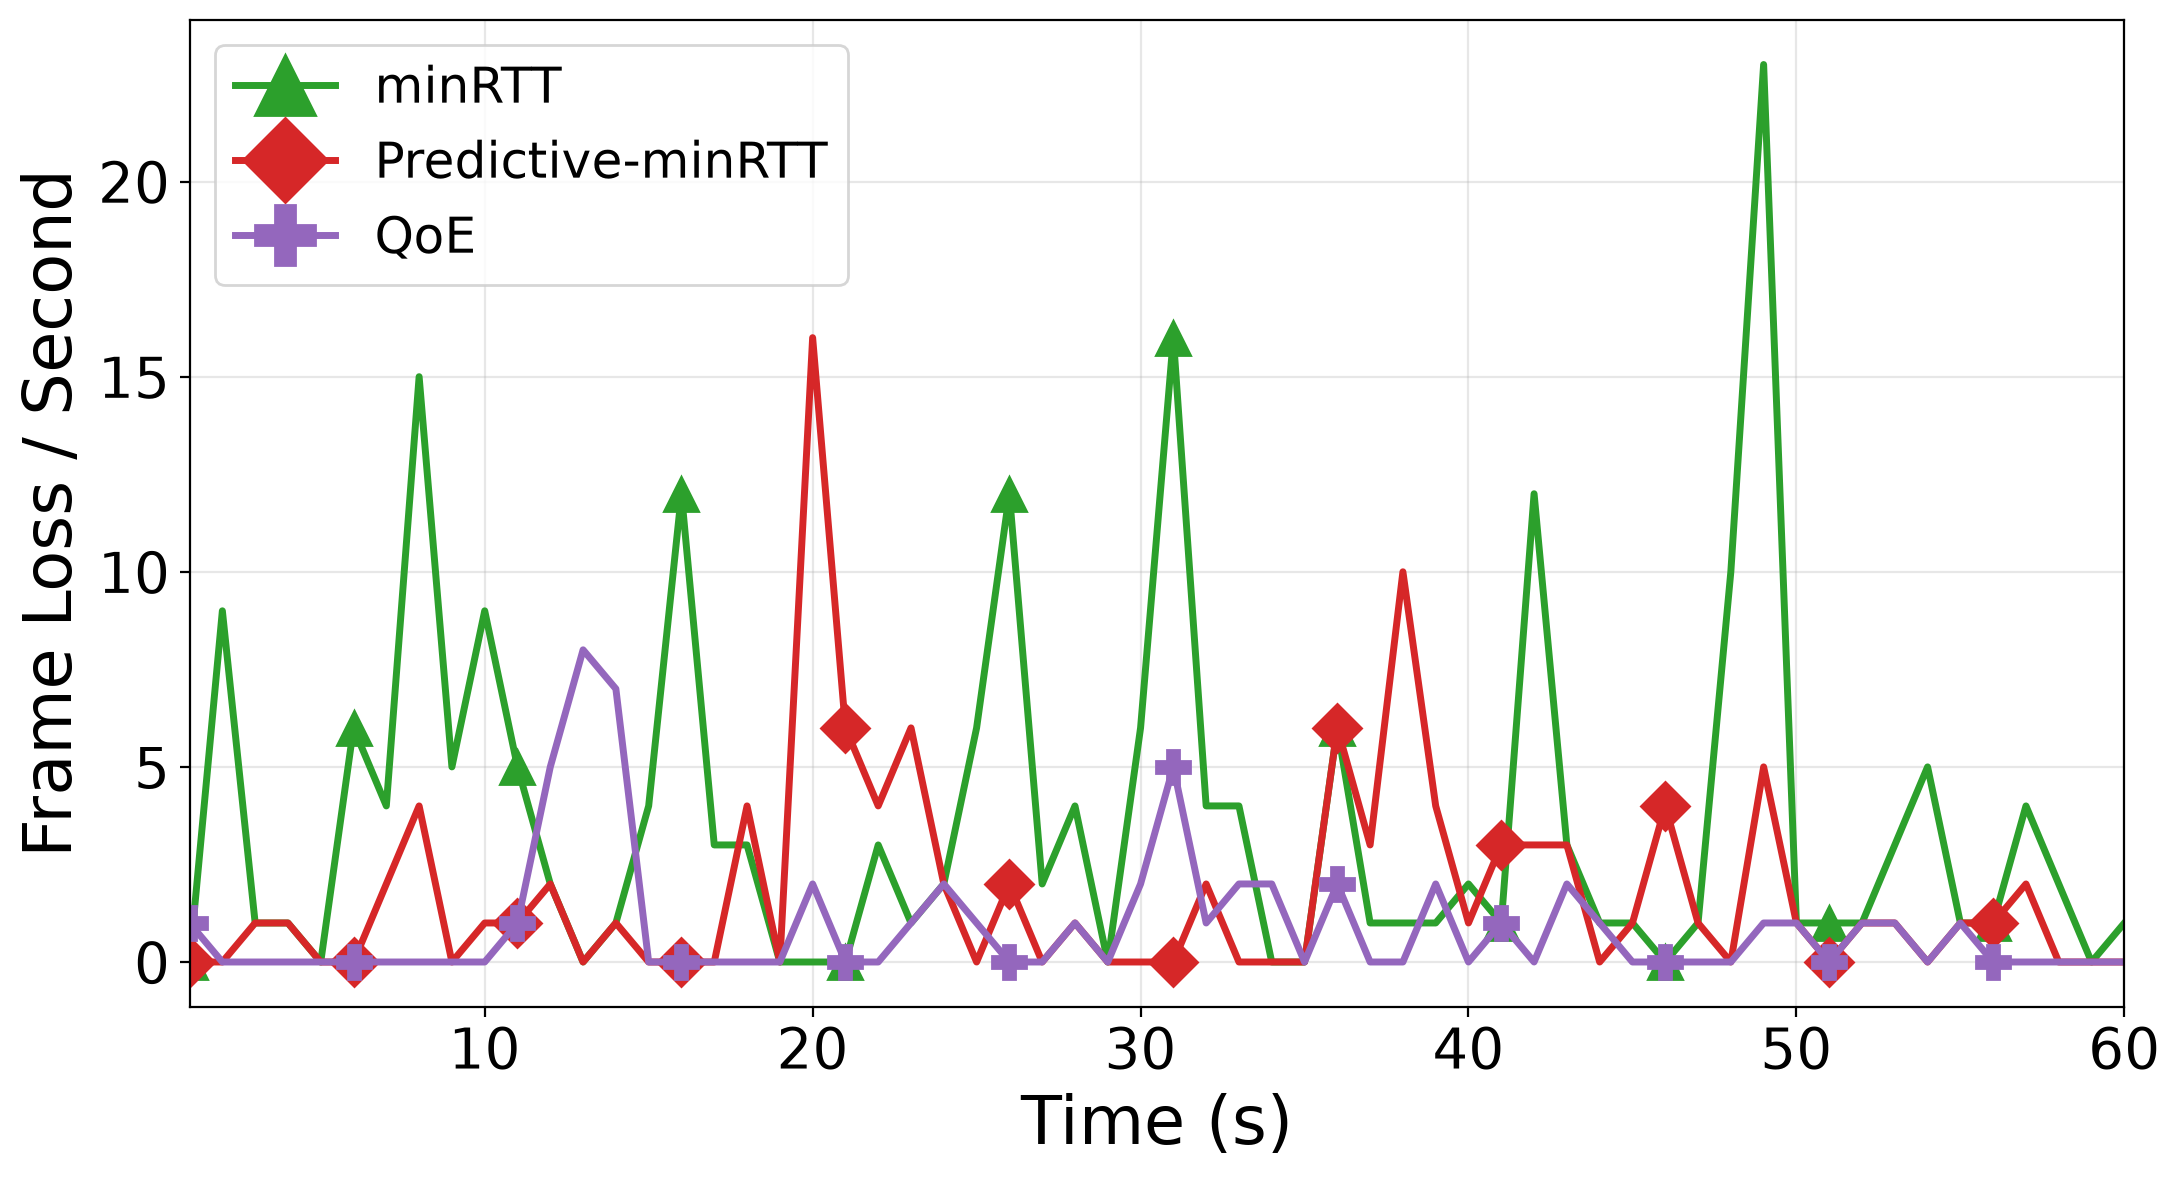
\includegraphics[width=\columnwidth]{images/frame_loss_schedulers.png}
        \caption{Packet scheduling comparison.}
        \label{fig:frame_loss_schedulers}
    \end{subfigure}

    \caption{Frame loss comparison across network paths and packet scheduling algorithms.}
    \label{fig:frame_loss_comparison}
\end{figure}


\begin{table*}[!htb]
    \centering
    \caption{Video streaming performance across network paths and packet scheduling algorithms. Average FPS, packet loss per second, frame loss per second, and IFA times. Median packet dispersion.}
    \label{tab:video_performance}
    \resizebox{\textwidth}{!}{%
    \begin{tabular}{|l||c|c|c|c|c|c|}
        \hline
        \textbf{Trial} &
        \textbf{FPS} &
        \textbf{Packet Loss (\%)} &
        \textbf{Frame Loss/s} &
        \textbf{Packet Disp. ($\mu$s)} &
        \textbf{IFA (ms)} &
        \textbf{Total Frame Loss} \\
        \hline
        \hline
        Starlink
            & 20.55
            & 32.26
            & 11.87
            & 324.81
            & 118.99
            & 712 \\
        \hline
        Quectel
            & 23.42
            & 12.66
            & 4.13
            & 265.68
            & 44.74
            & 248 \\
        \hline
        minRTT
            & 25.27
            & 9.98
            & 3.72
            & 248.26
            & 41.19
            & 223 \\
        \hline
        Predictive-minRTT
            & 25.08
            & 5.82
            & 1.78
            & 245.00
            & 41.63
            & 107 \\
        \hline
        QoE
            & 27.05
            & 15.86
            & 0.90
            & 239.84
            & 37.63
            & 54 \\
        \hline
    \end{tabular}%
    }
\end{table*}

\subsection{Intelligent Packet Scheduling}
\label{subsec:intelligent_scheduling}

Finally,  we evaluate the results of integrating our path-modeling framework with our intelligent packet scheduling defined in Section \eqref{sec:qoe_scheduler}. Starting with FPS, we see that it provides the most stable and highest frame rate throughout Fig. \eqref{fig:fps_schedulers}, with an average of 27 FPS. As seen in Fig. \eqref{fig:frame_loss_schedulers}, we see that the QoE-predictive scheduler provides a much more stable experience by significantly reducing the frame losses per second, with only 54 total frame losses, a reduction of $49.5\%-92.4\%$ compared to the others. We do notice higher packet loss per second, which requires further investigation and improvements to the scheduling algorithm. Lastly, as shown in Fig. \eqref{fig:ifa_comparison} and the table, we see the QoE-predictive scheduler having the closest IFA time to the expected 33.3\,ms IFA time. This is closer than the other schedulers, meaning that its frames are significantly less likely to be dropped by the application for being too late.

\begin{figure}[!htbp]
    \centering

    \begin{subfigure}[b]{\columnwidth}
        \centering
        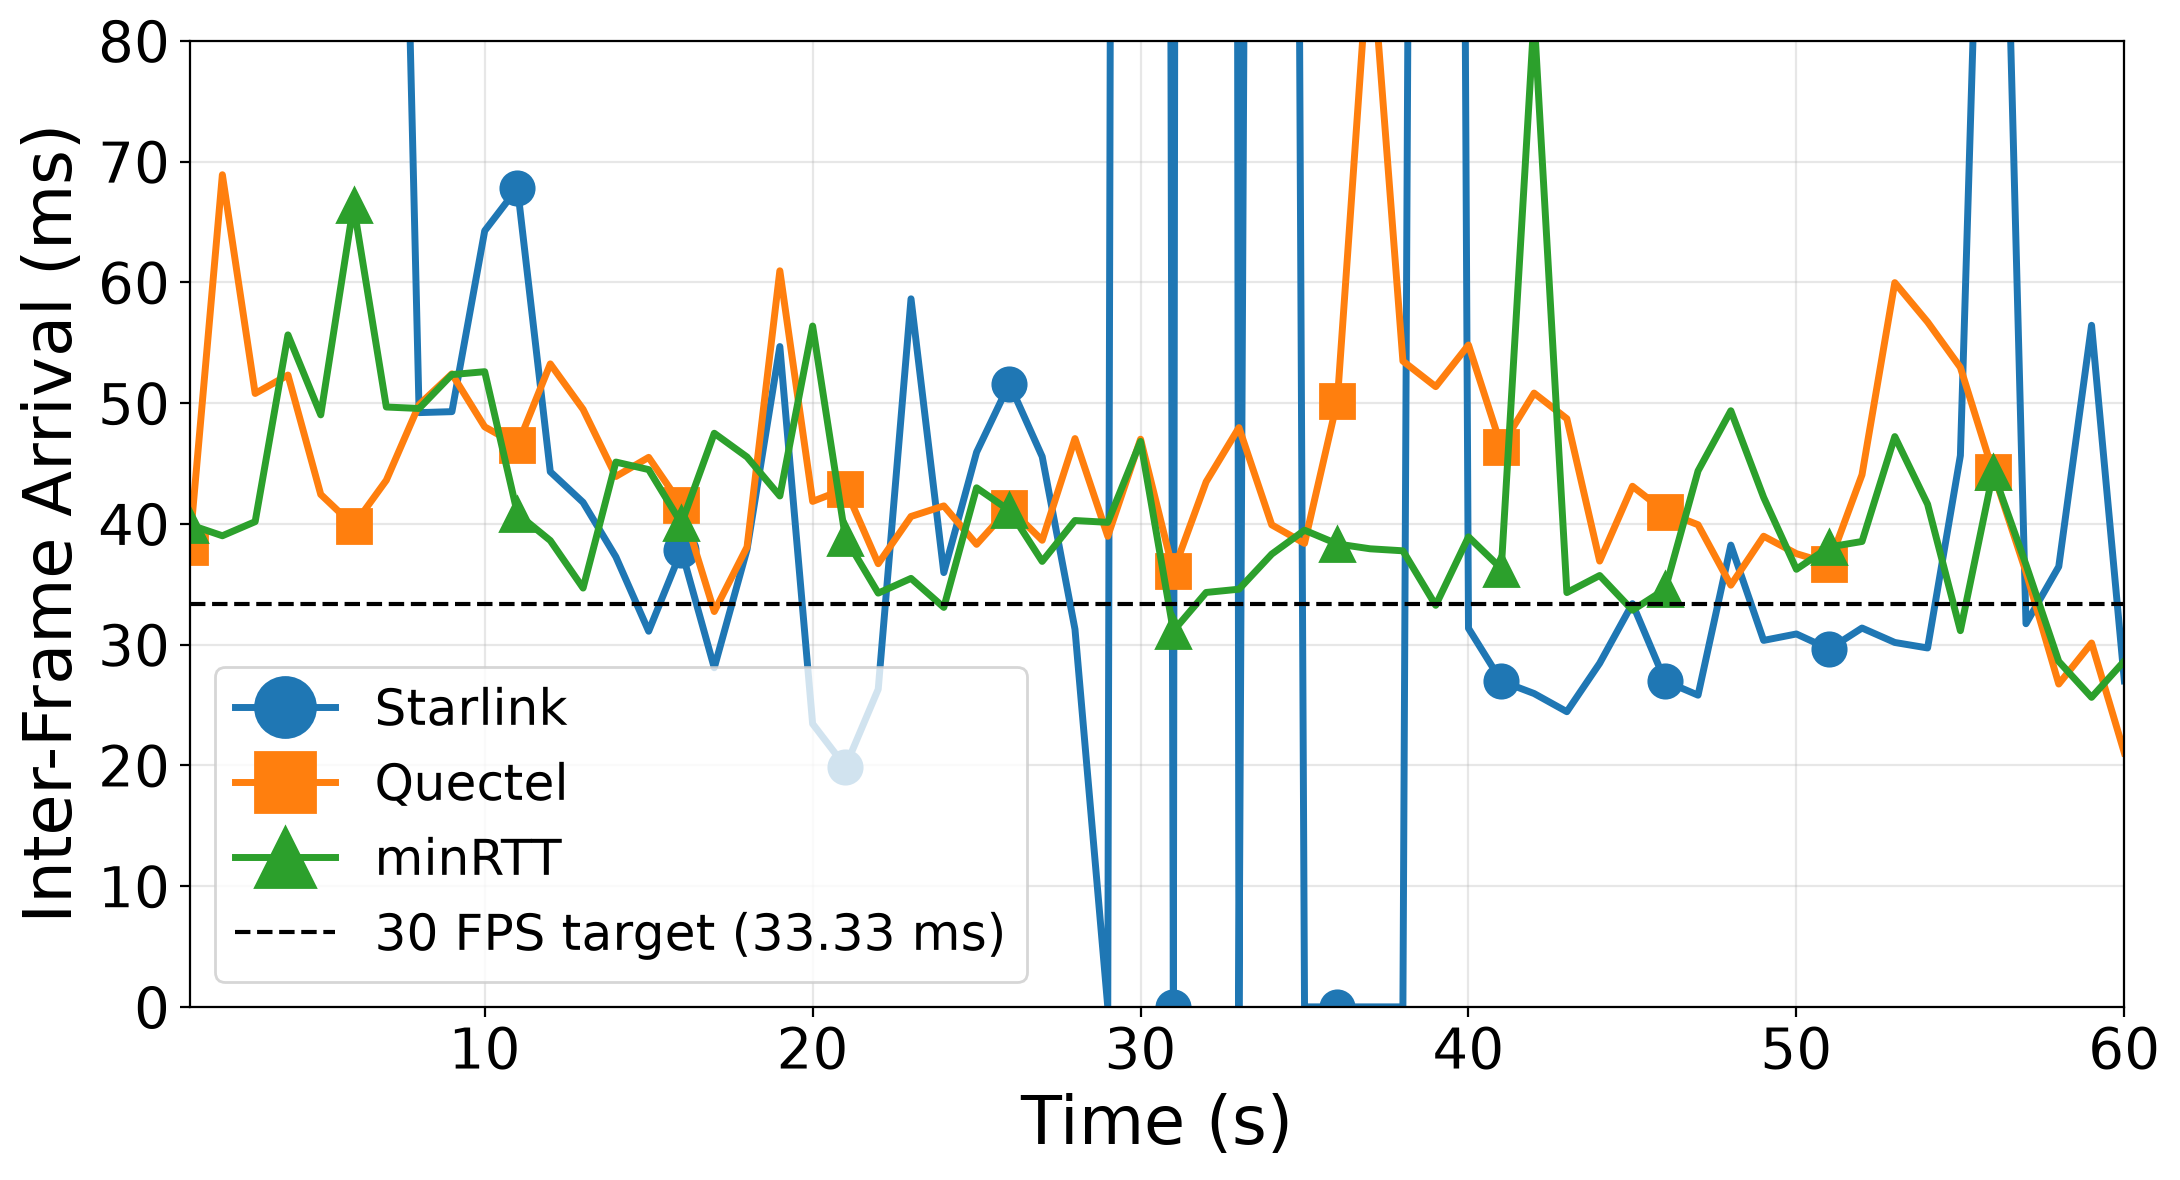
\includegraphics[width=\columnwidth]{images/ifa_paths.png}
        \caption{Starlink, Quectel, and minRTT.}
        \label{fig:ifa_paths}
    \end{subfigure}

    \vspace{0.5em}

    \begin{subfigure}[b]{\columnwidth}
        \centering
        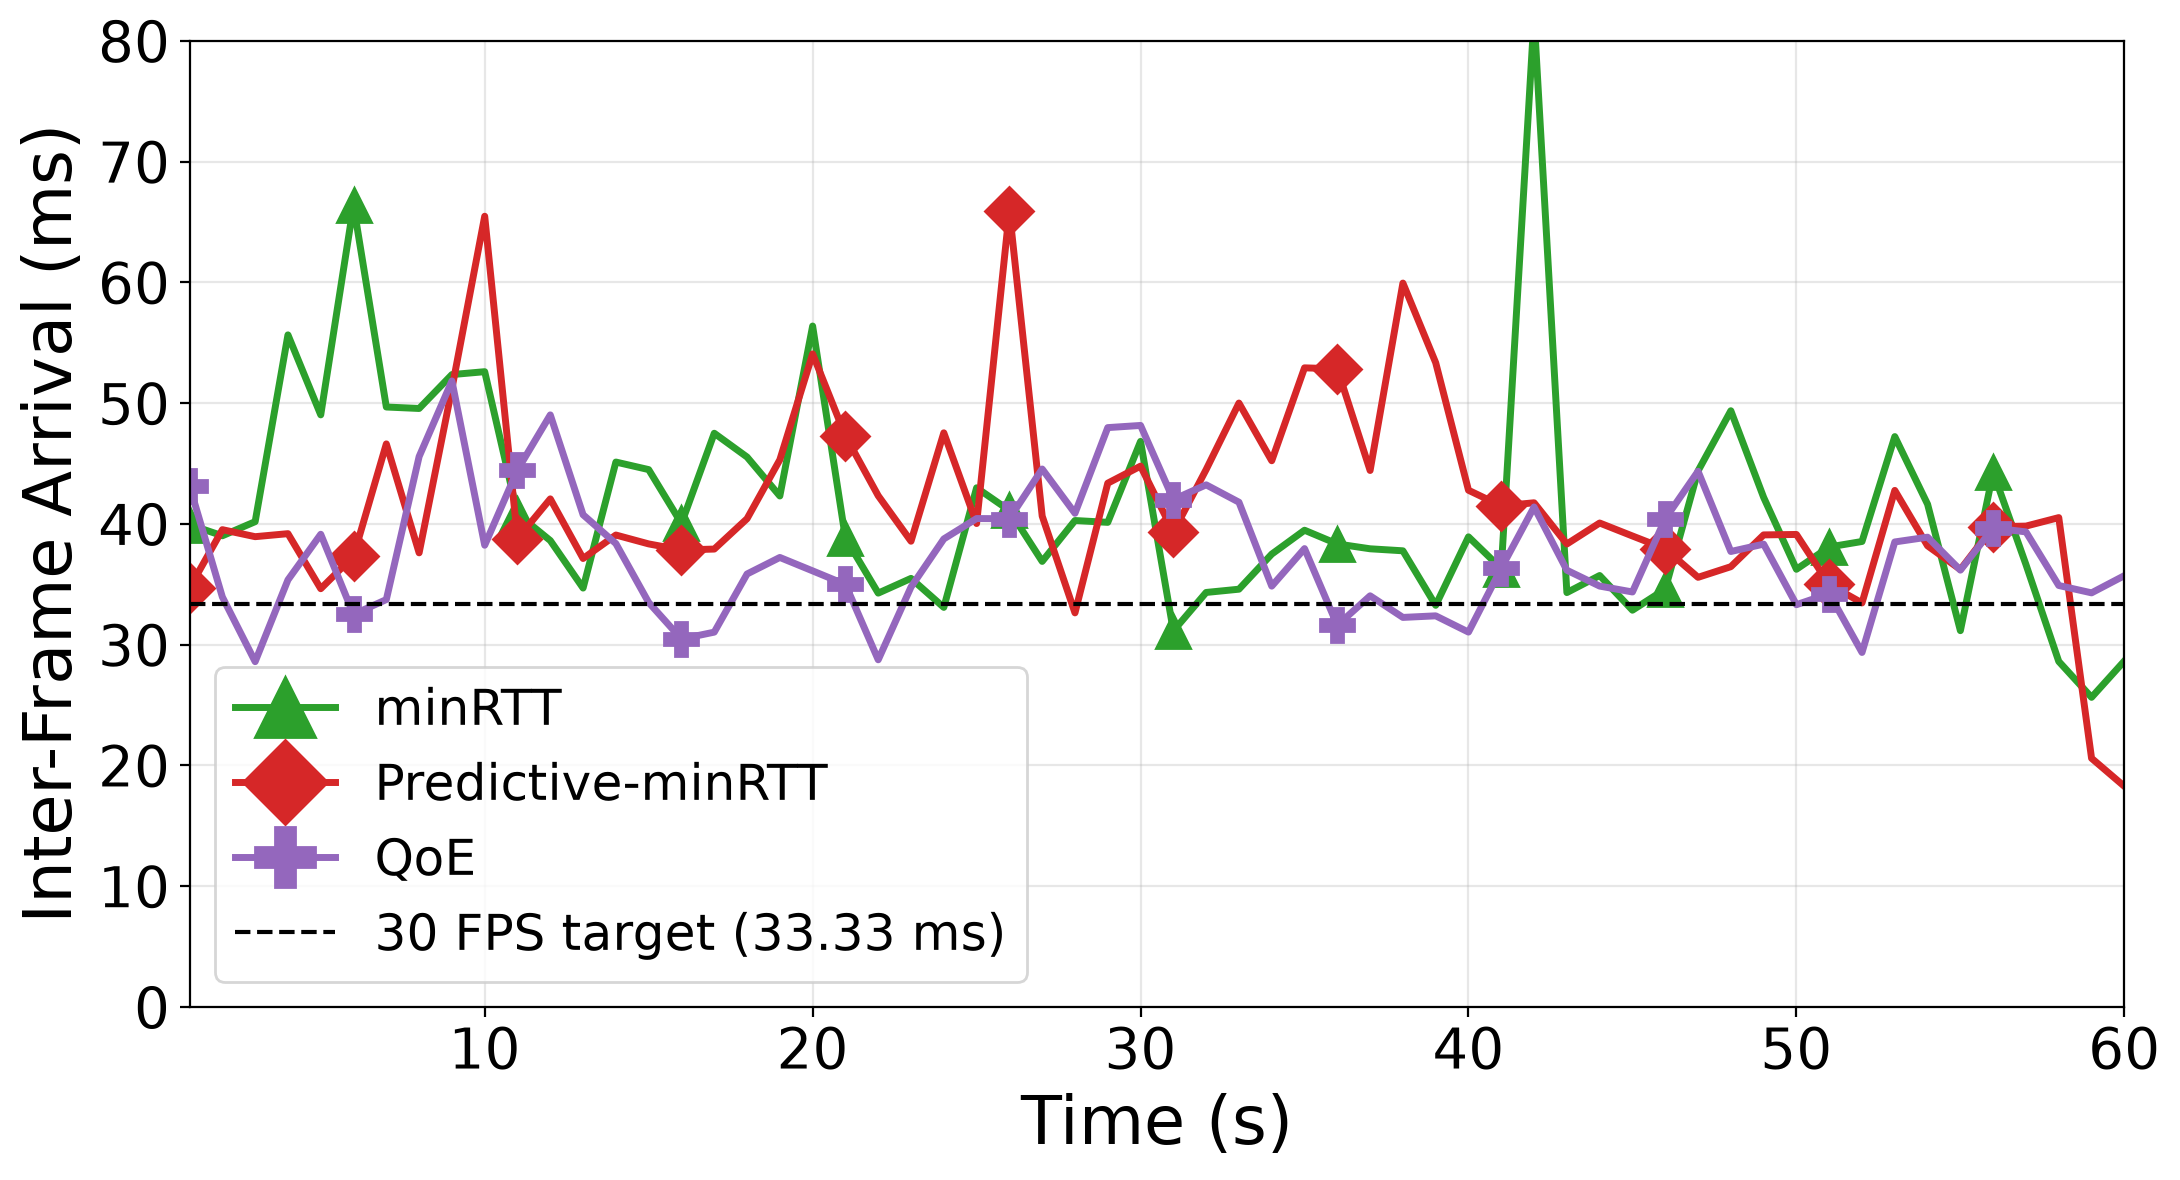
\includegraphics[width=\columnwidth]{images/ifa_schedulers.png}
        \caption{Packet scheduling comparison.}
        \label{fig:ifa_schedulers}
    \end{subfigure}

    \caption{Inter-frame arrival time comparison across network paths and packet scheduling algorithms.}
    \label{fig:ifa_comparison}
\end{figure}

% We next evaluate the results of integrating our path-modeling framework with an intelligent packet scheduling. Conventional multipath scheduling relies primarily on instantaneous or recently observed path statistics and is therefore inherently reactive to changes in network conditions. This limitation is particularly relevant in integrated terrestrial$-$satellite networks, where heterogeneous path dynamics can result in rapid variations in delay and reliability. The proposed prediction-assisted approach augments the measured path state with short-term QoS forecasts, enabling scheduling decisions to account for anticipated path variations.

% For each active path $p$, the modeling framework provides the predicted QoS state at prediction horizon $h$ as:
% \begin{equation}
%     \hat{\mathbf{q}}_{p}(t+h)
%     =
%     \left[
%         \widehat{\mathrm{RTT}}_{p}(t+h),
%         \widehat{J}_{p}(t+h),
%         \widehat{L}_{p}(t+h)
%     \right],
%     \label{eq:predicted_path_state}
% \end{equation}
% where $\widehat{\mathrm{RTT}}_{p}(t+h)$, $\widehat{J}_{p}(t+h)$, and $\widehat{L}_{p}(t+h)$ denote the predicted RTT, throughput, and packet-loss rate, respectively. 
% The predicted state is combined with the instantaneous path statistics maintained by the MPQUIC stack to characterize both the current and expected short-term conditions of each candidate path.

% The scheduler exploits this information to perform proactive packet allocation. 
% In particular, a path with favorable instantaneous statistics can be deprioritized when its predicted QoS indicates an impending degradation, whereas a path with improving predicted conditions can be selected before the improvement is fully reflected in the measured path statistics. 
% This behavior is particularly relevant to 5G$-$LEO multipath operation, where terrestrial radio variations and satellite-specific events, including handovers and changes in ground-segment conditions, may alter the
% relative quality of the available paths over short timescales.


\section{Limitation and Future Work}
\label{sec:limitations}

\subsection{Modeling}
Although the presented results demonstrate the potential of short-term link prediction for integrated satellite-terrestrial networks, several limitations remain. First, the current datasets are collected from a limited number of locations and network configurations. In particular, the terrestrial measurements primarily consider static 5G UEs, whereas mobility can introduce additional dynamics due to rapidly varying channel conditions, blockage, and handovers. Similarly, the available LEO measurements do not capture the full range of geographic locations, network loads, weather conditions, and satellite configurations that may be encountered in operational deployments. The OneWeb dataset is also more limited than the Starlink dataset, restricting the availability of cross-layer features and the extent to which the observed results can be generalized.

We will continue to research the latest modeling approaches to improve our current path models. This includes investigating adaptive prediction horizons, reduced feature sets, uncertainty-aware scheduling, and models that explicitly encode known network dynamics. The feature-ablation results of the last study suggest that a compact set of network-layer measurements may provide comparable or better performance than using all available telemetry, potentially reducing both measurement and inference overhead. Rather than treating predictions as deterministic values, the scheduler can additionally exploit prediction confidence to avoid aggressive path switching when model uncertainty is high. These extensions will enable the development of a practical prediction-aware multipath framework capable of adapting to the heterogeneous and rapidly evolving characteristics of integrated terrestrial and LEO satellite networks.

\subsection{Scheduling}
We will further refine and research intelligent scheduling algorithms to improve their performance. We note higher packet loss with our QoE-predictive scheduler, and visually in the recordings (not shown in this report) we observe more artifacts and discoloration in the video compared to other schedulers. Refinement of the algorithm and tuning the scheduling parameters to reduce packet reordering are also required to improve the scheduler (we notice an occasional spike in packet reordering that needs investigation).

Integrating our FEC mechanism into the scheduler and significant experimentation and tuning is also in our near-term future work. This integration will redefine how the scheduler algorithm will need to be modeled, due to the erasure coding blocks and the interchangeable nature of our selected RaptorQ erasure-coding mechanism. 

Lastly, we will look to include more network-level metrics from the liquid tunnel, for example, the amount of traffic sent over each path, in our final report.

\section{Conclusion}
\label{sec:conclusion}

This work demonstrated the potential of prediction-aware multipath scheduling for real-time applications in a heterogeneous 5G--LEO STIN. Using the Liquid Tunnel and a 4K 30~FPS video stream, predictive-minRTT reduced frame loss per second by 52\% compared with conventional minRTT, while the QoE-predictive scheduler achieved the highest average FPS (27.05), lowest frame loss (0.90 frames/s), and lowest total frame loss (54 frames).

These results show that incorporating path models to predict the path state can improve real-time application performance beyond reactive scheduling alone. However, the higher packet loss and observed packet-reordering behavior of the QoE-predictive scheduler indicate that further refinement is needed. Future work will focus on improving the scheduling policy, addressing reordering and loss, and evaluating the approach across broader network conditions.

% \section*{Acknowledgments}


%%
%% References
%%
\bibliographystyle{ACM-Reference-Format}
\bibliography{references}

\end{document}